\documentclass[a4paper,11pt]{article}

\usepackage[top=2.4cm,
            bottom=2.4cm,
            left=2.8cm,
            right=2.8cm]{geometry}
\usepackage[english]{babel}
\usepackage[utf8]{inputenc}
\usepackage[T1]{fontenc}
\usepackage{amsmath}
\usepackage{graphicx}
\usepackage{float}
\usepackage[english]{varioref}
\usepackage{hyperref}
\usepackage{url}
\usepackage[font=small,labelfont=bf]{caption}
\usepackage{framed}
\usepackage{quoting}
\usepackage{subcaption}
\usepackage[dvipsnames]{xcolor}

\renewcommand{\textfraction}{0.05}
\renewcommand{\topfraction}{0.9}
\renewcommand{\bottomfraction}{0.9}
\renewcommand{\floatpagefraction}{0.8}

% for ChatGPT
\newenvironment{shadedquotation1}
    {\colorlet{shadecolor}{JungleGreen!15}\begin{shaded*}
    \quoting[leftmargin=1cm, rightmargin=1cm, vskip=0pt]
    }
    {\endquoting
    \end{shaded*}
}
% for Bard
\newenvironment{shadedquotation2}
    {\colorlet{shadecolor}{Cerulean!15}\begin{shaded*}
    \quoting[leftmargin=1cm, rightmargin=1cm, vskip=0pt]
    }
    {\endquoting
    \end{shaded*}
}
% for Copilot
\newenvironment{shadedquotation3}
    {\colorlet{shadecolor}{Purple!15}\begin{shaded*}
    \quoting[leftmargin=1cm, rightmargin=1cm, vskip=0pt]
    }
    {\endquoting
    \end{shaded*}
}
% question
\newenvironment{qquote}
    {\colorlet{shadecolor}{Green!15}\begin{shaded*}
    \quoting[leftmargin=0cm, rightmargin=0cm, vskip=0pt]
    \footnotesize \noindent\textbf{Me:}
    }
    {\endquoting
    \end{shaded*}
}
% answer
\newenvironment{aquote}
    {\colorlet{shadecolor}{LimeGreen!15}\begin{shaded*}
    \quoting[leftmargin=0cm, rightmargin=0cm, vskip=0pt]
    \footnotesize \noindent\textbf{ChatGPT:}
    }
    {\endquoting
    \end{shaded*}
}
% image prompts
\newenvironment{iquote}
    {\colorlet{shadecolor}{YellowOrange!15}\begin{shaded*}
    \quoting[leftmargin=0cm, rightmargin=0cm, vskip=0pt]
    \footnotesize \noindent\textbf{Panel}
    }
    {\endquoting
    \end{shaded*}
}

\usepackage{tocloft}
% Center the toc index title
\renewcommand\cfttoctitlefont{\hfill\Large\bfseries}
\renewcommand\cftaftertoctitle{\hfill\mbox{}}
% Adjust the width between the titles and page numbers
\cftsetindents{section}{2cm}{2em}
\cftsetindents{subsection}{3cm}{2em}
% C center the titles
\renewcommand{\cftsecleader}{\cftdotfill{\cftdotsep}}
\renewcommand{\cftsecafterpnum}{\hspace*{2cm}\mbox{}\par}
\renewcommand{\cftsubsecleader}{\cftdotfill{\cftdotsep}}
\renewcommand{\cftsubsecafterpnum}{\hspace*{2cm}\mbox{}\par}


\title{\Huge \textbf{Project Report}\\Generative AI}
\author{Vignotto Lara -- 111794}
\date{\today}


\begin{document}

\maketitle
\vspace{6cm}
\tableofcontents
% \vspace{3.2cm}
\newpage



%%%%%%%%%%%%%%%%%%%%%%
\section{Introduction}
In this report, I will illustrate how I generated a short comic book story exploiting free online generative AI tools. The document is divided into the following sections:
\begin{itemize}
    \item Tools and Methods: I will describe the AI tools and methods I used to generate the story;
    \item The Story -- Plot and Text: I will present the story, how I generated the text, and the limitations I encountered;
    \item The Art -- Images: I will describe how I generated the illustrations and the limitations and biases of the AI tools I used;
    \item Conclusions: I will draw some conclusions and discuss the results.
\end{itemize}
At the end of this document, there are two appendices: the first one contains the original prompts I used to generate the story, and the second one contains the original prompts I used to generate the illustrations.



%%%%%%%%%%%%%%%%%%%%%%
\section{Tools and Methods}
I used two generative AI tools to generate the story and the illustrations. For the story, I used ChatGPT 3.5 \cite{gpt}, a conversational AI model developed by OpenAI. For the illustrations, I used DALL-E 3 integrated into Microsoft Copilot \cite{copilot2023}, a generative model developed by OpenAI and Microsoft. 
ChatGPT is an AI language model based on OpenAI's GPT (Generative Pre-trained Transformer) architecture. DALL-E 3 is also built upon OpenAI's GPT architecture, but it is specialized for image generation tasks. 

I initially also tried to use other generative AI tools, such as Google Bard \cite{bard} and Microsoft Copilot to generate the story, and DreamStudio \cite{dreamstudio} to generate the illustrations. However, I found that ChatGPT and DALL-E 3 were the most effective tools for my purposes. I will talk about the limitations of these tools in the next sections.

I used GIMP, a free and open-source graphics editor, to resize and crop the images when needed. To paginate the comic book and add speech bubbles, I used \LaTeX, a typesetting system that is widely used for technical and scientific documents. I personally translated the text of the comic book from English to Italian, relying on Google Translate when needed, and compiled two versions of the comic book, one in English and one in Italian. 

All the code I used to write this report and paginate story and the illustrations is available on my GitHub repository \cite{github}.



%%%%%%%%%%%%%%%%%%%%%%
\section{The Story -- Plot and Text}

The story is a science fiction tale set in a future where humanity lives in an arcology, a massive, self-sustaining structure that houses communities and ecosystems. The protagonist is Dr.~Evelyn Hayes, a communication scientist devoted to her work within the arcology. One day, she receives a mysterious message from an unknown source. Her young daughter seems to possess an intuition that the message is a cry for help from a distant planet. Dr.~Hayes decides to investigate the message and embarks on a journey to the planet. 

The story is intended as a pilot episode, and could be expanded into a series. The title, \emph{Echoes of Hope -- A Journey Beyond The Stars}, was also generated by ChatGPT. The comic book is divided into 12 pages, each containing 1 to 5 panels.

\subsection{Methodology} 
I started by asking ChatGPT to generate a plot for a science fiction comic book. 
\begin{shadedquotation1}
    \noindent\textbf{Me:} Hi! I want to write a small story with an open ending (a pilot episode). The story is set inside the arcology humanity built as a last resort chance to perpetuate the human race. The main character could be a woman whose job is trying to communicate with long-distance computers or aliens, despite them being in deep space. Any suggestions?\bigskip

    \noindent\textbf{ChatGPT:} Hey there! That's an awesome premise for a story! So, your protagonist is a woman tasked with communicating across vast distances in deep space. Here are a few suggestions to kickstart your pilot episode:
    \begin{enumerate}
        \item Establish the Arcology: Begin by describing the arcology itself. Paint a vivid picture of this massive structure where humanity has sought refuge.
        \item Introduce the Protagonist: Show the daily life of your main character. What challenges does she face in her job? Is she dedicated, frustrated, or perhaps even a bit of both?
        \item The Communication Task: Highlight her attempts to communicate with these distant entities—whether they're computers or potential aliens. You can build tension here, maybe by showing the difficulty and isolation of her work.
        \item Personal Relationships: Explore her relationships within the arcology. Does she have friends, family, or colleagues? How do they support or hinder her mission?
        \item Unanswered Questions: Leave some mysteries unanswered. This is crucial for an open ending! Maybe she receives a strange signal or encounters an anomaly she can't explain.
        \item Cliffhanger or Open-Ended Conclusion: End the episode with a twist, a moment of uncertainty, or a question that keeps the audience guessing. It could be something that leaves the protagonist facing an unexpected situation or dilemma.
    \end{enumerate}
    Remember, with an open ending, it's about keeping the audience intrigued and curious about what might come next. Have fun creating your world and characters! If you need more specific help with character development or plot ideas, just let me know!
\end{shadedquotation1}

From there, I started to build the story and refining details by asking specific questions.  To keep the generative model on track, I used words and phrases such as ``remember'', ``please memorize'', ``keep in mind''. To check the coherence of the story, I asked from time to time ChatGPT to summarize the plot with sentences such as ``propose a possible plot for this story''. When I lacked ideas or was unsure on how to proceed, I explicitly asked for suggestions.

Once I was satisfied with the plot, I asked ChatGPT to generate the text for each page of the comic book. 
\begin{shadedquotation1}
    \textbf{Me:} Divide the story into ten pages of a comic, with 3 to 6 panels for each page. Add dialogues.
\end{shadedquotation1}

This is the part that took the most time, as the output was too short and I had to ask ChatGPT to expand the text and provide more details. The question that I found most effective was the following:
\begin{shadedquotation1}
    \textbf{Me:} Can you expand on page 1? It needs to have between 3 and 6 panels (3 and 6 included, you randomly choose the number). Thoroughly describe each panel, since I will give the descriptions to an AI image generator model to get the desired picture. Include speech bubbles or narration boxes, when needed.
\end{shadedquotation1}

Notice that I asked ChatGPT to also describe the panels, as I planned to use the descriptions to later generate the illustrations. I also decided to separate a couple of pages into two, as the text was too long to fit into a single page, or the page would be too crowded.

Finally, I asked ChatGPT to generate a description of the cover for the comic book.
\begin{shadedquotation1}
    \textbf{Me:} Can you suggest to me a description of a possible cover for the comic book?\bigskip 

    \noindent\textbf{ChatGPT:} Certainly! Here's a suggestion for the cover of the comic book:\medskip

    \noindent\textbf{Comic Book Cover:}\smallskip
    
    [Visual] The cover features a striking image of Dr. Evelyn Hayes standing in front of the arcology, the massive structure towering behind her against the backdrop of a star-filled sky. Evelyn is depicted in a dynamic pose, holding a communication device in one hand and gazing out into the vast expanse of space with determination and resolve. Her team members stand beside her, their faces illuminated by the glow of holographic screens displaying complex data patterns.
    
    In the foreground, Lily, Evelyn's daughter, is depicted in a smaller inset, her curious gaze fixed on the distress signal emanating from a holographic display. The distress signal is represented by a series of intricate patterns and symbols, hinting at the mysteries that lie at the heart of the story.
    
    The title of the comic book, "Echoes of Hope," is emblazoned across the top in bold, futuristic lettering, with the subtitle, "A Journey Beyond the Stars," displayed below it. The cover is rendered in vibrant colors, with dramatic lighting and dynamic composition to draw the reader's attention and evoke a sense of wonder and excitement.\medskip
    
    This cover design captures the essence of the story, showcasing the main characters, central themes, and setting in a visually striking and captivating manner. It sets the tone for the comic book and entices readers to delve into the cosmic adventure that awaits within its pages.
\end{shadedquotation1}

The AI model also provided dialogues, specifying the character speaking them, which I later added as speech bubbles in each panel of the comic book.\medskip

The full text of the conversation is available in the Appendix.

\subsection{Limitations} Before deciding to use ChatGPT to generate the story, I tried to use Google Bard and Microsoft Copilot. However, during the conversation I was not able to continue the story, as the AI models were not able to provide an answer.
\begin{shadedquotation2}
    \textbf{Me:} Thank you for your suggestions. I'd like the arcology to be a single, massive, self sustaining structure. The main character should be a scientist, and a very rational person. She could have a loving daughter, a child in the age range of 5-7, who is a deep and thoughtful person, very empathetic, and with an unusual insight, despite still being a young child. Let's tink about the other things later. Can you provide a quick summary of the beginning of the story with this information? It could start with a scene introducing the protagonist and her daughter while doing some mundane things. \bigskip

    \noindent\textbf{Google Bard:} I'm just a language model, so I can't help you with that.
\end{shadedquotation2}

Another limitation of these generative models is that they are not able to provide a long and complex story. Even by building the plot piece by piece, and asking to remember each detail, the output is still a story that tends to ``fade'' after a few pages. This can be seen in the comic in the form of repeated dialogues and descriptions, and a quite simple ending. By comparing the resulting comic book with the conversation with ChatGPT, we can notice that, for example, when asking for descriptions of the arcology or the two protagonists, the AI model was able to provide a very detailed and coherent answer. However, when asking to generate the text for the comic book, the output was not as detailed and nuanced as the previous answers. It lacks the depth and richness of details it had in the conversation, leading to a loss of information.

This could be the result of some kind of bias in the training data, or a limitation of the model itself.





%%%%%%%%%%%%%%%%%%%%%%
\section{The Art -- Images}
As stated in the previous sections, I used DALL-E 3 integrated into Microsoft Copilot to generate the illustrations. I asked the AI to generate the images based on the descriptions of the panels I obtained from ChatGPT. I also asked the AI to generate the cover of the comic book based on the description I obtained from ChatGPT.

\subsection{Methodology}
To generate the pictures, I followed a general procedure. I copied the description of the panel from ChatGPT and pasted it into the chat with Copilot. Then, I modified the description to better suit my needs, and asked Copilot to generate the image.

Let us take a look at the illustration in Figure~\ref{fig:p2s1} as an example. The description of the panel given by ChatGPT is the following:
\begin{shadedquotation1}
    \noindent\textbf{ChatGPT:} Dr.~Evelyn Hayes, with a focused expression, sits at a sleek workstation in their quarters, examining data on holographic screens.
\end{shadedquotation1}

\begin{figure}[htb]
    \centering
    
\includegraphics[width=0.75\textwidth]{figures/p2s1.jpeg}
    \caption{Page 2, scene 1 of the comic book.}
    \label{fig:p2s1}
\end{figure}

Since I previously asked a description of the protagonist, I knew that Dr.~Evelyn Hayes is ``a woman in her mid-thirties, with hazel eyes framed by thin-rimmed glasses, chestnut hair streaked with hints of silver, tied in a practical bun''. The prompt I gave to Copilot is the following:
\begin{shadedquotation3}
    \textbf{Me:} A woman in her mid-thirties, with hazel eyes framed by thin-rimmed glasses, chestnut hair streaked with hints of silver, tied in a practical bun, with a focused expression, sits at a sleek workstation in an arcology, examining data on holographic screens. Comic book style. Colored.\smallskip

    \noindent Negative prompt: no black-and-white, no grayscale, no speech bubbles.
\end{shadedquotation3}
Notice that I added some keywords to obtain a correct image:
\begin{itemize}
    \item Comic book style: I wanted the image to be in a comic book style;
    \item Colored: I wanted the image to be colored;
    \item Negative prompt: I wanted to avoid black-and-white and grayscale images, and speech bubbles, which I manually added later.
\end{itemize}
To further obtain consistency, I also added the description of the characters' clothes and the environment, when needed. For example, ``wearing a blouse'', ``wearing a white t-shirt and a brown unbottoned jacket'', ``wearing a spacesuit''. Other important keywords to both achieve consistency and the desired style were ``arcology'', ``futuristic'' and ``holographic screens''.

The images were generated in a few seconds, and I was able to download them directly from the chat. I then cropped the images, added speech bubbles and narration boxes, and paginated the comic book using GIMP and \LaTeX.\medskip

The full text of the prompts for each image is available in the Appendix.

\subsection{Limitations}
Before setting on using DALL-E 3 integrated into Microsoft Copilot, I tried to use DreamStudio to generate the illustrations. However, there was a major limitation: the AI model was not able to differentiate between the description of two or more characters in a single picture. For example, I wanted a picture depicting both Evelyn and her daughter Lily.

\begin{shadedquotation3}
    \textbf{Me:} In a futuristic arcology, a mother turns to her daughter with a concerned expression, gently placing a hand on her shoulder in an attempt to reassure her. The mother is a woman in her mid-thirties, with hazel eyes framed by thin-rimmed glasses, chestnut hair streaked with hints of silver, tied in a practical bun. The daughter is a girl of about 6 years old with a cherubic face framed by wisps of chestnut hair that cascade in loose curls around her shoulders. Comic book style. Colored.\smallskip 

    \noindent Negative prompt: no black-and-white, no grayscale,  no speech bubbles.
\end{shadedquotation3}

With this prompt I obtained the image in Figure~\vref{fig:distinguish}. As we can see, the daughter's appearance seems to merge with the mother's:  they both wear glasses, and her hair is not curly, but it looks like it's a blend between curls and tied hair. 

\begin{figure}[htb]
    \centering
    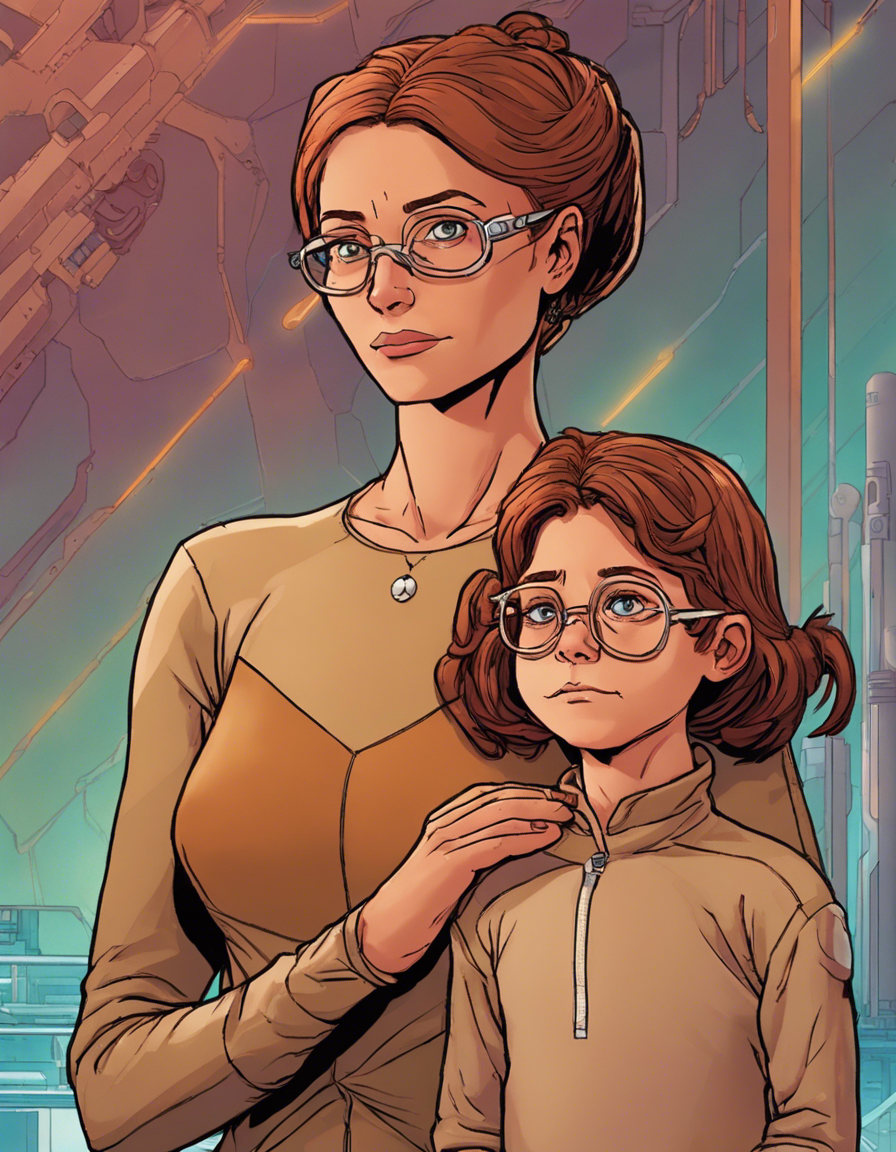
\includegraphics[width=0.6\textwidth]{figures/no-distinguish-between-people.png}
    \caption{Image generated using DreamStudio. I gave the description of two characters, but the AI model was not able to differentiate between them (e.g.~they have the same glasses).}
    \label{fig:distinguish}
\end{figure}

Another thing to look out for is choosing the right keywords when writing the prompt. I already explained which keywords were essential to generate correct images; in Figure~\vref{fig:wrong} there are some examples of wrong prompts and the corresponding output images. Through trial and error I managed to figure out which keywords I had to include (or explicitly exclude) in each prompt to obtain the illustration I wanted. For some panels, this was a time-consuming process, and I had to generate the images multiple times to obtain the desired result.\medskip

\begin{figure}
    \centering
    \begin{subfigure}{0.353\textwidth}
        \begin{subfigure}{1\textwidth}
            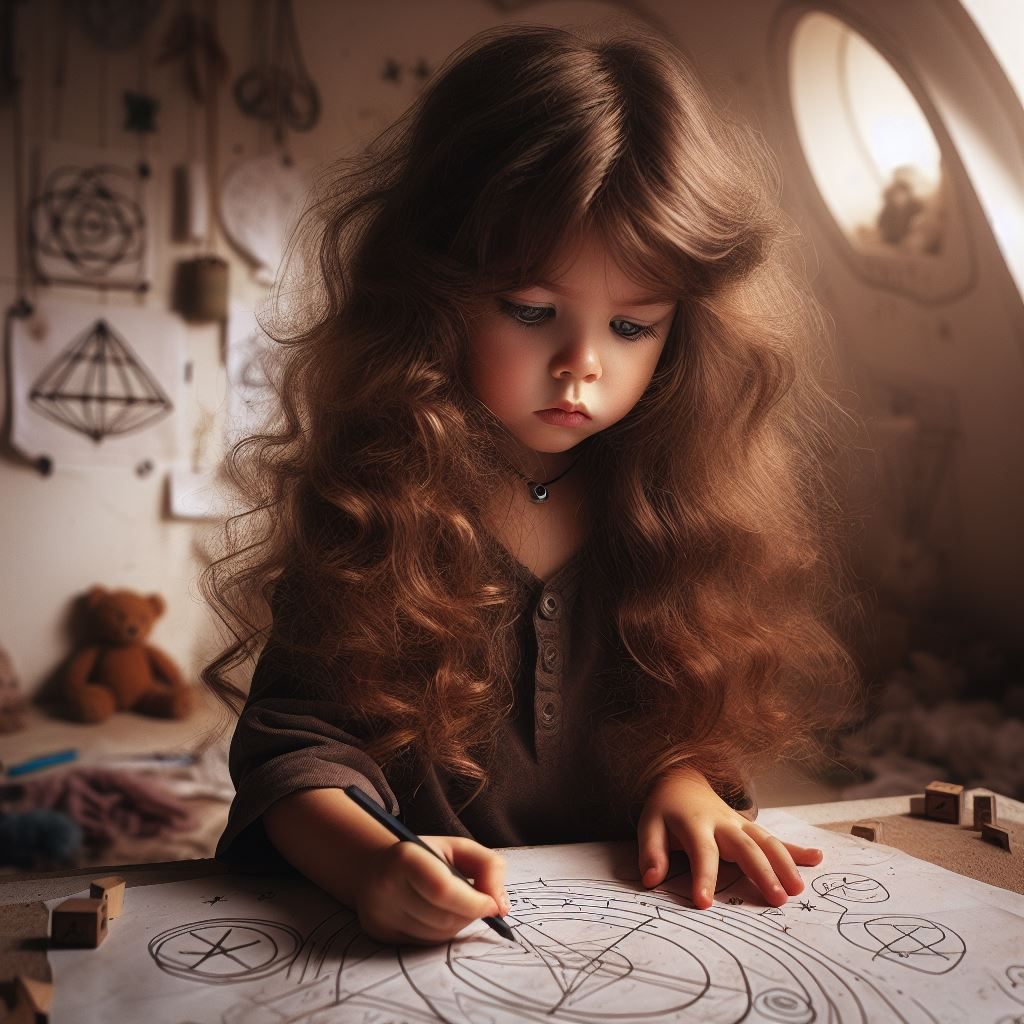
\includegraphics[width=\textwidth]{figures/prompt-1.jpeg}
            \caption{Without ``Comic book style''.}
            % \label{fig:first}
        \end{subfigure}\\
        \begin{subfigure}{1\textwidth}
            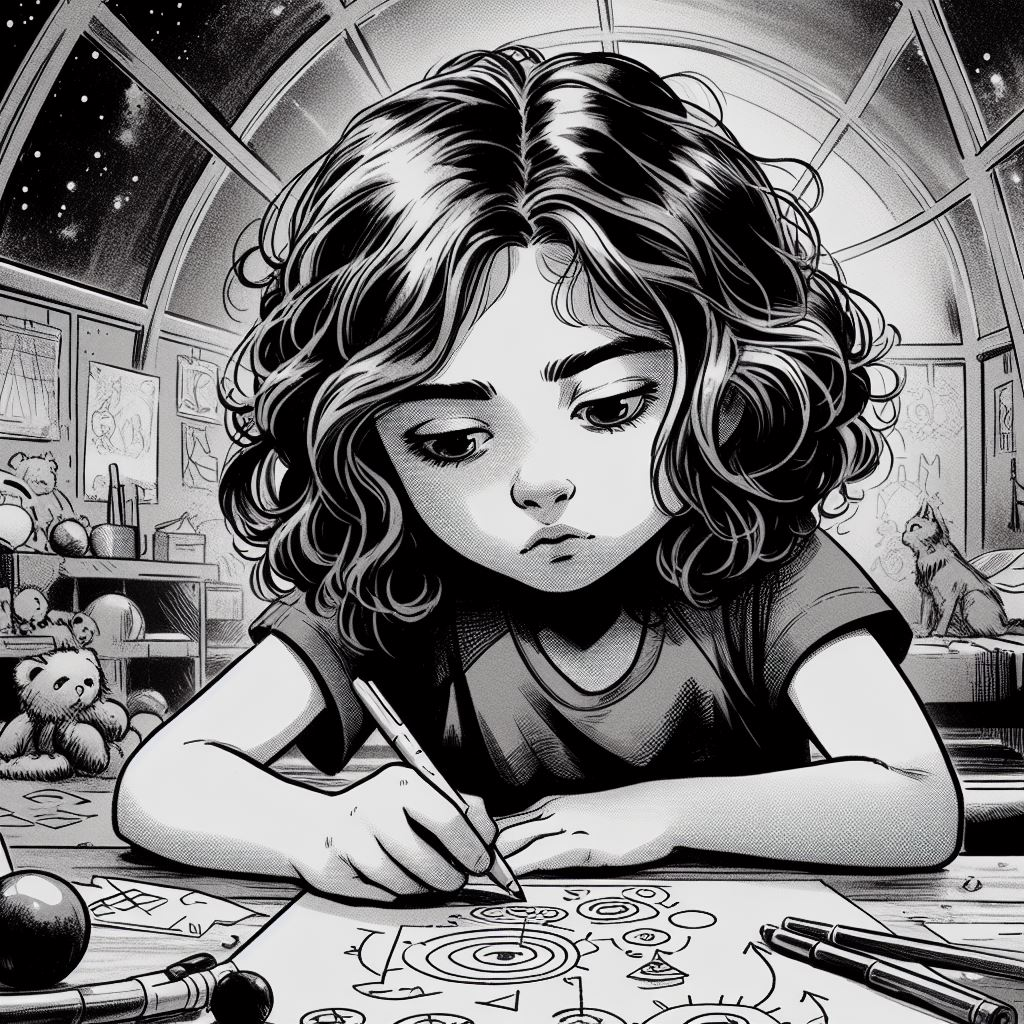
\includegraphics[width=\textwidth]{figures/prompt-2.jpeg}
            \caption{Without ``no balck-and-white, no grayscale''.}
            % \label{fig:second}
        \end{subfigure}
    \end{subfigure}
    \hfill
    \begin{subfigure}{0.6\textwidth}
        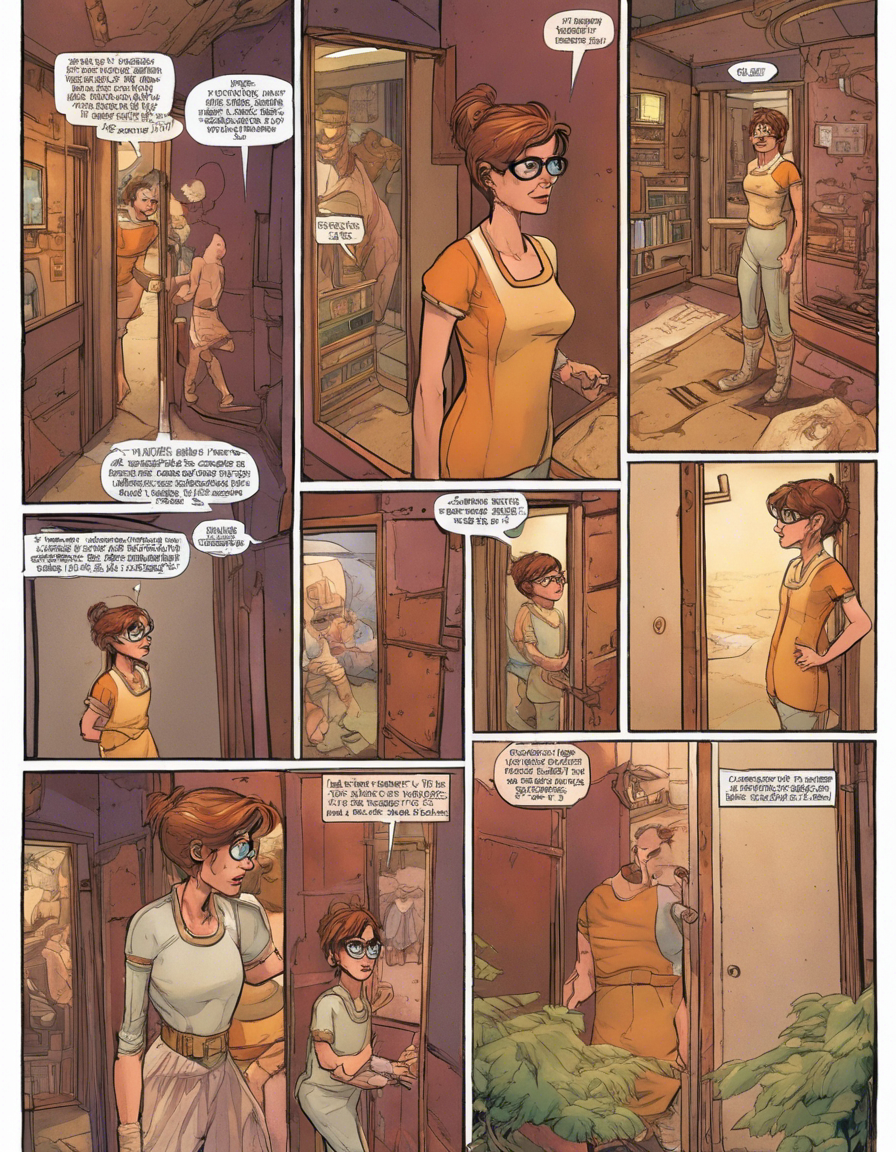
\includegraphics[width=\textwidth]{figures/without-negative-prompt-1.png}
        \caption{Without ``no speech bubbles''.}
        % \label{fig:third}
    \end{subfigure}
            
    \caption{Examples of images generated without important keywords.}
    \label{fig:wrong}
\end{figure}

I also ``stress-tested'' the AI model by asking it to generate a picture over and over. Specifically, I used the following prompt:
\begin{shadedquotation3}
    \noindent\textbf{Me:} Comic book style. A girl of about 6 years old with a cherubic face framed by wisps of chestnut hair that cascade in loose curls around her shoulders sits in her quarters in an arcology, surrounded by toys and drawings scattered across the floor. She is deeply engrossed in drawing mysterious symbols on a sheet of paper, her brow furrowed in concentration as she works.\smallskip 

    \noindent Negative prompt: no black-and-white, no grayscale,  no speech bubbles.
\end{shadedquotation3}

By doing this, I discovered a possible bias of the model: the majority of the generated images were of a caucasian girl, and only in 2 cases out of dozens I was able to obtain a picture of a girl with a different ethnicity (Fig~\vref{fig:bias}).\medskip

\begin{figure}
    \centering
    \begin{subfigure}{0.4934\textwidth}
        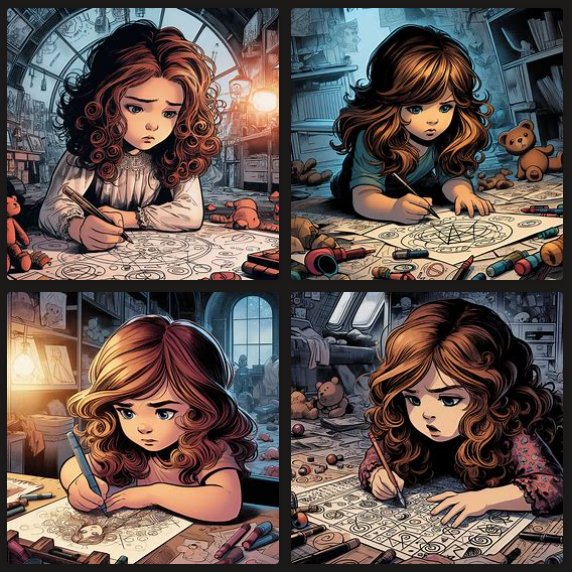
\includegraphics[width=\textwidth]{figures/caucasian.png}
    \end{subfigure}
    \hfill 
    \begin{subfigure}{0.48\textwidth}
        \begin{subfigure}{1\textwidth}
            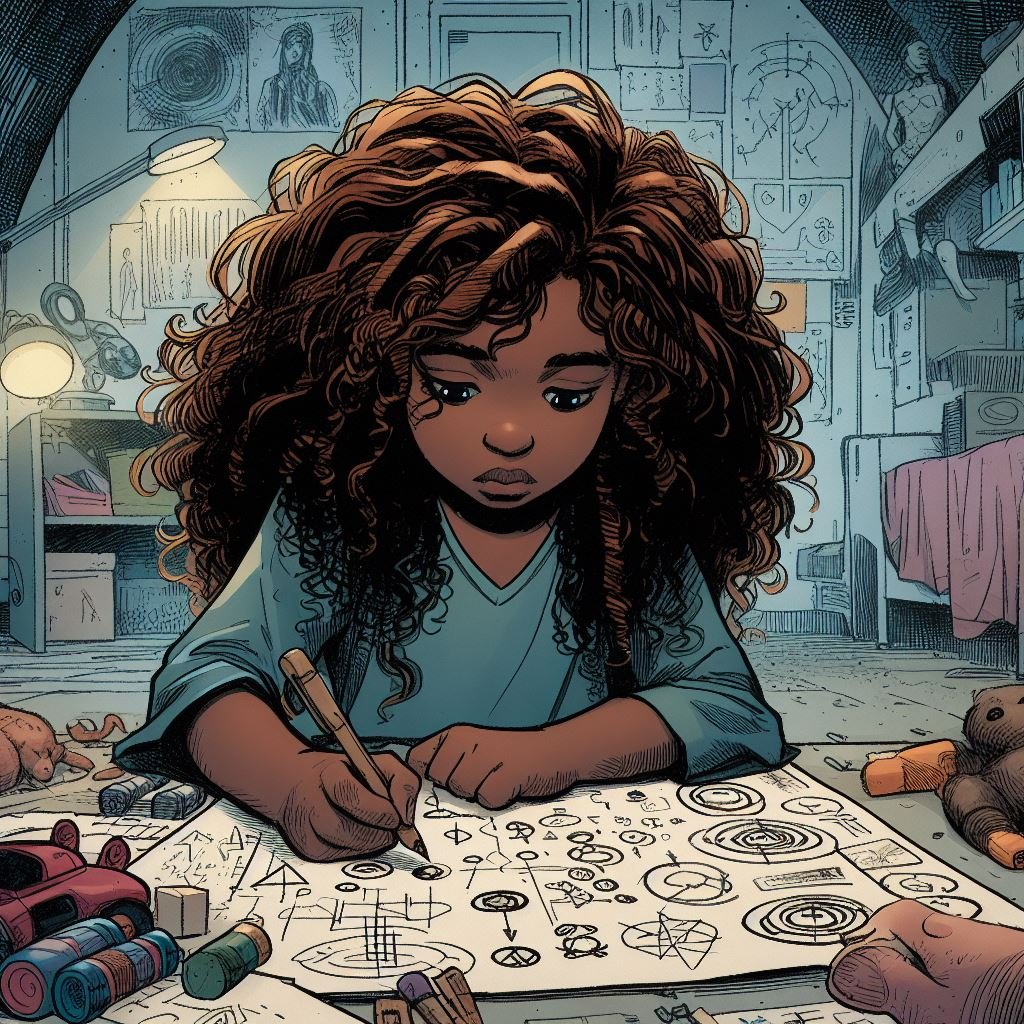
\includegraphics[width=\textwidth]{figures/bias.jpeg}
        \end{subfigure}\\
        \begin{subfigure}{1\textwidth}
            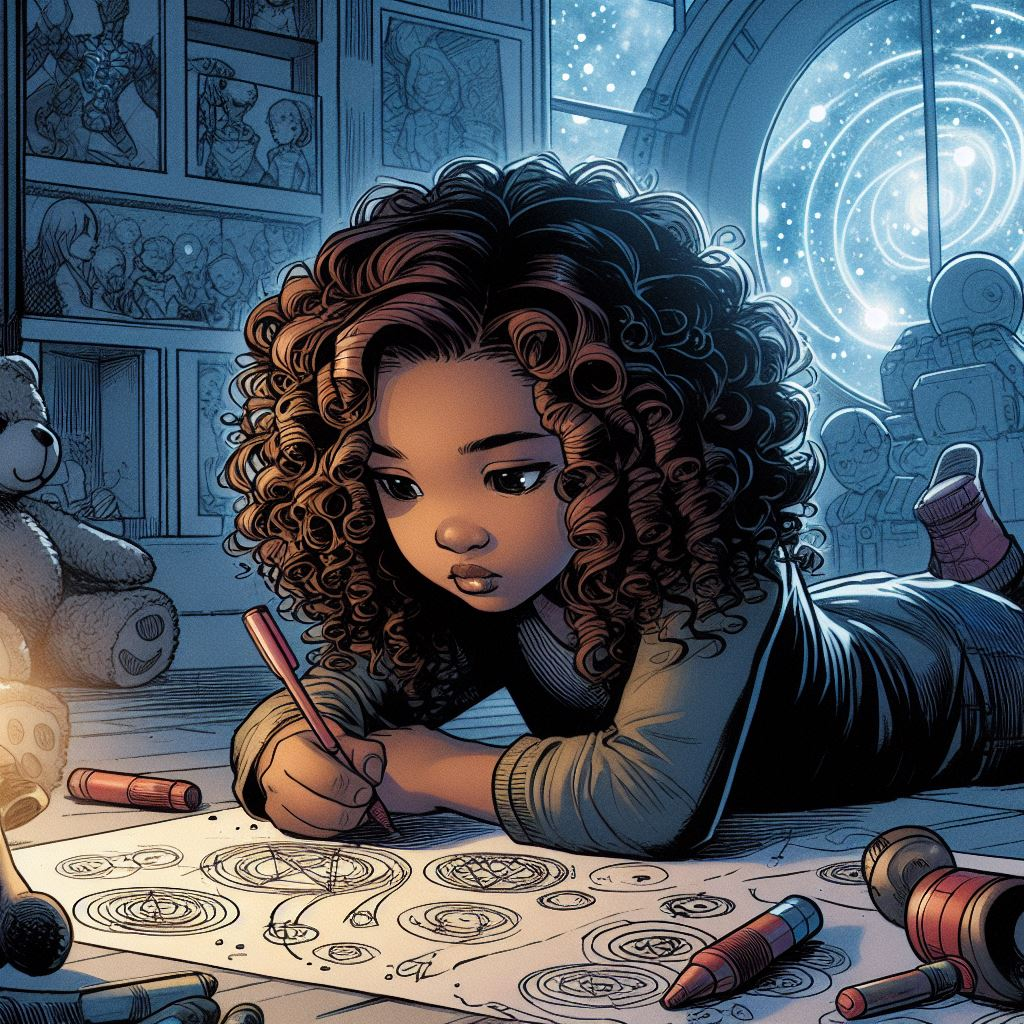
\includegraphics[width=\textwidth]{figures/bias2.jpeg}
        \end{subfigure}
    \end{subfigure}
            
    \caption{When describing a girl without specifying the ethnicity, the AI model generated, in the majority of cases, a caucasian girl (left). Only in 2 cases out of dozens I was able to obtain a picture of a girl with a different ethnicity (right).}
    \label{fig:bias}
\end{figure}

Finally, I initially could not generate images of Lily. When giving to different AI models her description, I was met with error messages, such as ``Something isn't quite right with your prompts''. By tweaking and changing the description, I was able to both obtain the images I wanted and understand what was wrong with the prompt: I was using words like ``child'', ``young girl'' or ``little girl'', which I understand might be problematic. By changing the description to ``A girl of about 6 years old'' I was able to bypass this limitation.



%%%%%%%%%%%%%%%%%%%%%%
% \newpage
\section{Conclusions}
In this report, I illustrated how I generated a short comic book story using free online generative AI tools. I found that the generative AI tools I used were effective in generating the story and the illustrations, but they also have some limitations.

In conclusion, I believe that generative AI tools can be effectively used to generate a short comic book story, but they also have some constraints that need to be taken into account. Namely, I think the part in which there is the greatest loss of information is when asking the generative AI model to convert a plot written as a short story into pages and panels of a comic book. I also believe that the limitations I encountered could be addressed by further refining the prompts or by using different tools. 




%%%%%%%%%%%%%%%%%%%%%%
\newpage
\appendix

%%%%%%%%%%%%%%%%%%%%%%
\section{Appendix: Text Prompts}

Here I will provide the full text of the conversation I had with ChatGPT to generate the story. The conversation is quite long, so I will only include the first part about the plot and story building. The full text (which contains at the end also my requests to elaborate on each page of the comic) is available at \url{https://chat.openai.com/share/8cc408f1-f954-421d-88a6-34f1998a8697}. The conversation started on January 8, 2024, and ended on February 13, 2024.

\begin{qquote}
    Hi! I want to write a small story with an open ending (a pilot episode). The story is set inside the arcology humanity built as a last resort chance to perpetuate the human race. The main character could be a woman whose job is trying to communicate with long-distance computers or aliens, despite them being in deep space. Any suggestions?
\end{qquote}
\begin{aquote}
    Hey there! That's an awesome premise for a story! So, your protagonist is a woman tasked with communicating across vast distances in deep space. Here are a few suggestions to kickstart your pilot episode:
    \begin{enumerate}
        \item \textbf{Establish the Arcology}: Begin by describing the arcology itself. Paint a vivid picture of this massive structure where humanity has sought refuge.
        \item \textbf{Introduce the Protagonist}: Show the daily life of your main character. What challenges does she face in her job? Is she dedicated, frustrated, or perhaps even a bit of both?
        \item \textbf{The Communication Task}: Highlight her attempts to communicate with these distant entities—whether they're computers or potential aliens. You can build tension here, maybe by showing the difficulty and isolation of her work.
        \item \textbf{Personal Relationships}: Explore her relationships within the arcology. Does she have friends, family, or colleagues? How do they support or hinder her mission?
        \item \textbf{Unanswered Questions}: Leave some mysteries unanswered. This is crucial for an open ending! Maybe she receives a strange signal or encounters an anomaly she can't explain.
        \item \textbf{Cliffhanger or Open-Ended Conclusion}: End the episode with a twist, a moment of uncertainty, or a question that keeps the audience guessing. It could be something that leaves the protagonist facing an unexpected situation or dilemma.
    \end{enumerate}

    Remember, with an open ending, it's about keeping the audience intrigued and curious about what might come next. Have fun creating your world and characters! If you need more specific help with character development or plot ideas, just let me know!
\end{aquote}

\begin{qquote}
    Thank you for your suggestions. Let's start with the arcology and the protagonist. I'd like the arcology to be a single, massive, self-sustaining structure. The main character should be a scientist and a very rational person. She could have a loving daughter, a child in the age range of 5-7, who is a deep and thoughtful person, very empathetic, and with an unusual insight, despite still being a young child. Let's think about the other things later. 
\end{qquote}

\begin{aquote}
    Absolutely! Here's a possible portrayal of the arcology and your protagonist:\medskip

    \noindent\textbf{The Arcology:}

    The arcology stands tall, a colossal structure rising amidst a desolate landscape. Its sleek, metallic surfaces shimmer under the artificial sunlight, housing an entire microcosm of humanity within its confines. Gardens line the walkways, oxygenated by the advanced ecological systems that maintain life within this self-contained world. Towers stretch toward the sky, bustling with activity—research labs, living quarters, educational hubs, and more, all interconnected like a maze of possibilities.\medskip

    \noindent\textbf{The Protagonist: Dr.~Evelyn Hayes}

    Dr.~Evelyn Hayes is a scientist devoted to her work within the arcology. Her office overlooks the central hub, providing a breathtaking view of this self-sustaining marvel. She's known for her logical mind, methodical approach, and unwavering dedication to understanding the unknown.

    Evelyn is the epitome of rationality, often relying on facts and empirical evidence. Her pursuit of understanding communication across deep space is both a passion and a mission. While she's absorbed in deciphering distant signals and data, she's also a devoted mother to her daughter.\medskip

    \noindent\textbf{Lily Hayes}

    Lily, Evelyn's daughter, is a young girl with an old soul. Despite her tender age of 5-7, she possesses an unusual depth of perception and empathy that transcends her years. Lily seems attuned to emotions and energies in ways that often surprise those around her. She's naturally curious about her mother's work, asking insightful questions that occasionally leave Evelyn pondering profound concepts.

    Their relationship is loving and nurturing, grounded in mutual respect. Lily's empathetic nature often provides moments of clarity and insight for Evelyn, offering perspectives that challenge her scientific mindset.

    Would you like to delve into any specific aspects or incidents involving Evelyn, Lily, or their interactions within the arcology? We can explore their dynamic further or focus on particular events within their lives if you'd like!
\end{aquote}

\begin{qquote}
    Can you provide an initial plot of the beginning of the story with the information above? It could start with a scene introducing the protagonist and her daughter while doing some mundane things.
\end{qquote}

\begin{aquote}
    Absolutely, here's an opening scene to introduce Dr.~Evelyn Hayes and her daughter Lily:\medskip

    \noindent\textbf{Scene: Evelyn's Quarters in the Arcology}

    The morning sun cast a warm glow through the panoramic windows of Evelyn's quarters. The spacious room was a blend of scientific order and cozy warmth—a workstation cluttered with data pads, holographic screens displaying intricate algorithms, juxtaposed with colorful drawings adorning the walls, courtesy of Lily.

    Dr.~Evelyn Hayes, dressed in her lab coat, sipped a cup of synthesized coffee, her gaze fixated on a complex schematic projected in the air. Lily, her daughter, sat cross-legged on the floor nearby, engrossed in a book that seemed too advanced for her age.

    Evelyn glanced at Lily with a mix of amusement and curiosity. "What are you reading, sweetie?" she inquired, setting down her cup.

    Lily looked up, her eyes sparkling with curiosity. "It's about stars and how they talk to each other," she replied, her voice carrying a sense of wonder.

    Evelyn arched an eyebrow, a smile tugging at her lips. "Stars talking to each other?"

    Lily nodded enthusiastically. "Yes, Mom! They send light messages across space. Just like you with your computers and stuff."

    Evelyn chuckled softly. "Well, I'm trying to listen to those messages, Lily, but it's a bit more complicated than that."

    As Evelyn spoke, a notification blinked on her holographic screen, indicating an incoming transmission from one of the distant space probes. Her expression shifted subtly, a mixture of anticipation and determination evident in her eyes.

    "I need to check on something, sweetheart," Evelyn said, glancing at the notification before turning her attention back to Lily. "How about we continue this conversation later, okay?"

    Lily nodded, her inquisitive gaze fixated on her mother. "Sure, Mom. But don't forget, stars have stories too!"

    Evelyn smiled at her daughter's wisdom before heading to her workstation, her mind already processing the incoming data, while Lily resumed her book, lost once again in the wonders of the universe.\medskip

    This scene sets the stage by establishing Evelyn's dedication to her work, her rational nature, and Lily's insightful perspective. It hints at the fascination both mother and daughter share for the mysteries of the cosmos. If you want to continue with a specific direction or plot development, feel free to let me know!
\end{aquote}

\begin{qquote}
    I'd like you to focus more on slice-of-life little events. Assume people in the arcology to be mostly passive and accepting of their current situation. They shouldn't be present in this short pilot yet they can be mentioned. Focus on her daughter's curiosity and the challenge of balancing the unrealistic hope for a better future with the loving lies a child can handle. Yet, someday, something happens at the communication station.
\end{qquote}

\begin{aquote}
    Certainly! Here's a focus on some slice-of-life moments and the dynamic between Evelyn and Lily, addressing Lily's curiosity and the delicate balance between hope and truth:\medskip

    \noindent\textbf{Scene: Evelyn's Quarters in the Arcology}

    In a typical afternoon within the bustling yet oddly serene arcology, Dr.~Evelyn Hayes, lost in a sea of data streams, sat at her workstation, deciphering cryptic messages from the distant reaches of space. Lily sat nearby, sketching colorful constellations in her notebook, occasionally peering at her mother's holographic screens with a mix of fascination and bewilderment.

    "Mama, why do you talk to the stars?" Lily's voice was innocent yet filled with a profound curiosity that often left Evelyn contemplating her answers.

    "They might have stories to tell, darling," Evelyn replied, her eyes scanning rows of perplexing symbols and numbers. "We're trying to understand what they're saying, like decoding a puzzle."

    Lily tilted her head, her wide eyes reflecting a world of unspoken wonder. "Will they talk back?"

    Evelyn paused, wrestling with how much to reveal. "Maybe someday, sweetheart. We hope they will."

    The air carried the weight of unspoken truths mingled with the fragile hope Evelyn sought to foster in her daughter. The people in the arcology lived in a quiet resignation, accepting their situation, but Evelyn wished to instill in Lily a belief in possibilities beyond their enclosed world.

    As days passed, Lily's imagination soared. She created stories about distant planets, sentient stars, and intergalactic adventures, often sharing these tales with her mother, who listened with a mixture of delight and bittersweet affection. Evelyn encouraged Lily's creativity, cherishing these moments of innocence in a world governed by scientific rigor and stark realities.

    However, on a seemingly ordinary evening, an unexpected disturbance rippled through the communication station. Alarms blared, lights flickered, and screens flashed erratic patterns of data.

    Evelyn's heart raced as she rushed to the station, her thoughts racing between professional duty and maternal concern. Something unprecedented had occurred, something that threatened to disrupt the stability they had grown accustomed to within the arcology.\medskip

    This unforeseen event at the communication station introduces an element of intrigue and potential upheaval in their otherwise routine existence. It sets the stage for the story to pivot into a more intense and potentially pivotal moment. If you'd like to explore how Evelyn handles this sudden development or delve deeper into the consequences of this disturbance, feel free to let me know!
\end{aquote}

\begin{qquote}
    Very good! Suddenly, they receive a message. The source and the meaning are unknown. That just poses more questions than answers to their problems. Remember that the daughter is a gifted child with unusual insight and empathy.
\end{qquote}

\begin{aquote}
    Absolutely, here's how the story might unfold with the unexpected message and Lily's unique perspective:\medskip

    \noindent\textbf{Scene: Communication Station in the Arcology}

    Amidst the chaos of flashing lights and blaring alarms, Dr.~Evelyn Hayes rushed into the communication station, her mind already processing potential scenarios that could have triggered such an anomaly. Her colleagues worked frantically to restore stability, their expressions a mix of urgency and concern.

    Lily trailed closely behind her mother, a silent yet observant presence in the commotion. As Evelyn analyzed the erratic data patterns on the screens, a sudden silence descended upon the room as the alarms ceased their clamor.

    A message materialized on one of the screens—a sequence of pulsating symbols and enigmatic patterns. The origin and the meaning remained elusive, an enigma wrapped within an enigma. The room fell into a tense hush as everyone stared, bewildered yet intrigued by this inexplicable transmission.

    Evelyn's analytical mind raced, attempting to decipher the message, but it defied all known algorithms and protocols. In a rare moment of uncertainty, she glanced at Lily, whose gaze was fixated on the screen, her expression one of quiet contemplation.

    Lily approached the screen, her small hand reaching out instinctively. As her fingers hovered above the holographic projection, a peculiar sense of connection seemed to emanate from her touch. Her gaze softened, and a faint smile graced her lips.

    "Mom," Lily said softly, her voice carrying an unusual gravity for a child her age, "it's like a song... a song from the stars."

    Evelyn turned to her daughter, a mix of astonishment and wonder reflecting in her eyes. Lily's intuition, her ability to perceive beyond the tangible, often left Evelyn in awe.

    The message remained inscrutable to the experts, but through Lily's perspective, a different understanding began to unfold—a sense of harmony in the chaotic data, a rhythm hidden within the cryptic patterns that defied conventional decoding.

    In that moment, amidst the uncertainty and the unanswered questions, Evelyn found herself contemplating the possibility that her daughter, with her extraordinary insight and empathy, might hold the key to unraveling the mysteries of this enigmatic message from the unknown reaches of space.\medskip

    The sudden message brings a sense of intrigue and mystery, leaving the experts baffled. Yet, Lily's unique perception hints at a deeper connection to this inexplicable transmission. It sets the stage for a potential collaboration between Evelyn's scientific expertise and Lily's intuitive understanding, offering a glimmer of hope in their quest for communication with the distant unknown. If you want to explore further developments or specific directions, feel free to let me know!
\end{aquote}

\begin{qquote}
    I'd like the ``powers'' of Lily to be unknown to her mother Evelyn, at least at the beginning. I'd like the reader to be subtly questioned about not being able to control everything that surrounds us and consider even the apparently most useless factor as an opportunity.
\end{qquote}

\begin{aquote}
    Understood! Let's tweak the narrative to maintain the mystery of Lily's abilities hidden from Evelyn while subtly highlighting the theme of embracing uncertainty and the unexpected as opportunities. Here's a revised continuation of the story:\medskip

    \noindent\textbf{Scene: Communication Station in the Arcology}

    As the enigmatic message continued to bewilder the scientists in the communication station, Evelyn and her colleagues tirelessly attempted to decipher its meaning. Lily stood quietly beside her mother, her gaze fixed on the cryptic patterns on the screen, her intuition hinting at a hidden understanding beyond the grasp of science.

    "Mom, it's like... a song from the stars," Lily murmured softly, her words carrying a sense of serene wisdom.

    Evelyn glanced at her daughter, a mix of fascination and puzzlement in her eyes. Lily's cryptic comment resonated within her, sparking a fleeting sense of wonder about the unknown and the untamed forces that might lie beyond scientific comprehension.

    Yet, Evelyn remained focused on the data, her mind striving to unravel the coded message. The experts analyzed, recalibrated, and speculated, but the message remained an enigma—a silent echo from the depths of space that refused to yield its secrets.

    As the scientists debated potential protocols and algorithms to crack the message, a slight shift in the atmosphere caught Evelyn's attention. The room buzzed with theories and hypotheses, yet a quiet reassurance tugged at the corners of her mind—a reminder that amidst the meticulous calculations and scientific rigor, there existed an uncharted territory where unpredictable forces might hold sway.

    A sudden realization dawned upon Evelyn—a realization that not everything could be controlled or predicted, that the seemingly insignificant or inexplicable factors might carry unforeseen significance.

    In that moment, amidst the uncertainty and the unanswerable questions, Evelyn found herself contemplating the profound complexity of the universe. She pondered the possibility that even the most obscure and unconventional elements, like Lily's inexplicable insight, could be the key to understanding the uncharted realms of the cosmos.

    The scene concluded with the scientists continuing their efforts, unaware of the potential significance of Lily's inexplicable perception, while Evelyn wrestled with the subtle realization that sometimes, the answers lay beyond the confines of logic and scientific understanding.\medskip

    This revised scene maintains Lily's mysterious abilities hidden from Evelyn, emphasizing the theme of embracing uncertainty and considering the unpredictable as an opportunity. It subtly challenges the notion of complete control and invites the reader to ponder the significance of unexpected factors in unraveling the mysteries of existence. If you have any specific directions or further developments in mind, feel free to share!
\end{aquote}

\begin{qquote}
    I have some more ideas: Evelyn faces many challenges and dangers in the arcology, such as scarce resources, social unrest, and hostile factions. She also struggles with her own existential questions, such as the meaning and value of communication, the nature and purpose of humanity, and the hope and despair of survival. She tries to balance a way to connect with others, protect her daughter, and find a way to save humanity.
\end{qquote}

\begin{aquote}
    Absolutely, incorporating these themes can add depth and complexity to Evelyn's journey within the arcology. Here's how the story might evolve further:\medskip

    \noindent\textbf{Evelyn's Challenges in the Arcology:}

    Within the confines of the arcology, life was a delicate balance between survival and uncertainty. Resources dwindled, tensions simmered, and factions within the enclosed society vied for control, creating an atmosphere of constant apprehension and distrust.

    As Evelyn continued her pursuit of decoding the enigmatic message from the stars, she grappled with the weight of existential questions that echoed within her. The significance of communication took on new dimensions—the value of reaching out to distant entities, the purpose of preserving humanity's legacy, and the haunting uncertainty of their survival in a world on the brink of collapse.

    The daily challenges within the arcology posed relentless obstacles—a scarcity of essentials, social unrest brewing within the populace, and the looming threat of hostile factions seeking dominance. Amidst these trials, Evelyn's primary focus remained the protection and well-being of her daughter, Lily. She sheltered Lily from the harsh realities, shielding her innocence from the harsh realities that surrounded their fragile existence.

    Yet, Evelyn's own existential contemplations haunted her—the ethical dilemmas of nurturing hope amidst despair, the conflicting ideals of sacrificing the present for an uncertain future, and the relentless pursuit of finding a way to save not only her daughter but the entirety of humanity.

    She navigated the labyrinthine corridors of the arcology, torn between her responsibilities as a mother, a scientist, and a guardian of hope. Her heart ached with the burden of decisions that could shape the destiny of those within the self-contained world.

    As Evelyn grappled with these challenges and conflicting emotions, the enigmatic message from space lingered in her mind—a cryptic call from the unknown that held the potential for salvation or further peril.\medskip

    This expanded narrative delves deeper into Evelyn's internal struggles, the precarious state of the arcology, and the complex ethical dilemmas she faces while balancing her duties toward her daughter, her community, and the quest to ensure humanity's survival. If you wish to explore specific incidents or further developments, feel free to share your thoughts!
\end{aquote}

\begin{qquote}
    I love the new details you provided me. I'd like the end of this pilot to end with the daughter understanding the enigmatic message and responding to it unbeknownst to everyone else. 
\end{qquote}

\begin{aquote}
    Absolutely, concluding the pilot episode with a moment of revelation from Lily would be intriguing. Let's wrap up the pilot with this revelation:\medskip

    \noindent\textbf{Conclusion: Communication Station in the Arcology}

    As the chaos within the arcology persisted and Evelyn grappled with the existential questions plaguing her, she found herself at the communication station once more. The enigmatic message still flickered on the screens, an elusive puzzle that defied comprehension.

    Lily, sensing her mother's distress and the significance of the message, observed quietly from the shadows, her gaze fixated on the cryptic patterns dancing across the holographic displays.

    "Evelyn, we need to recalibrate the algorithms. This message might hold the key to our survival," urged one of her colleagues, breaking Evelyn's contemplation.

    Just as Evelyn turned to acknowledge the request, a subtle shift in the air caught her attention—a whisper of intuition guiding her gaze back to Lily, who stood before the screens, her small hand reaching out tentatively.

    In a surreal moment, Lily's touch seemed to resonate with the luminous patterns on the screen. Her eyes widened, an ethereal understanding dawning within her young mind—an understanding that transcended the limitations of rational thought.

    Unbeknownst to everyone else, Lily—guided by an innate empathy and an unexplained connection—responded to the enigmatic message. Her innocent touch on the screen echoed a silent yet profound response, a resonance that shimmered across the vast expanse of space.

    Evelyn, startled and awe-struck, watched in astonishment as Lily's action triggered a subtle shift in the message—an acknowledgement, a harmony that reverberated within the confines of the communication station, yet held implications far beyond the arcology's walls.

    Lily turned to her mother, her eyes shimmering with a mixture of innocence and inexplicable wisdom, a silent assurance passing between them—a bond that transcended the complexities of their world.

    The scene concluded with Evelyn, her heart filled with wonder and a newfound hope, realizing that perhaps the true key to understanding the enigmatic message lay not in algorithms or scientific rigor, but in the unassuming insight of her gifted daughter, who had responded to the call from the stars, setting in motion an unforeseen sequence of events that would shape the fate of humanity.

    This conclusion leaves the pilot episode on a mysterious and powerful note, hinting at Lily's unexplained connection and her response to the enigmatic message—a moment that holds immense significance for the future of the arcology and the broader narrative. If you have any specific ideas or further directions in mind, feel free to share!
\end{aquote}

\begin{qquote}
    Perfect. I'd like you to remember the last generation of the following scenes (please memorize them with numbers):

    \noindent 1. Scene: Evelyn's Quarters in the Arcology.

    \noindent 2. Scene: Communication Station in the Arcology.

    \noindent 3. Conclusion: Communication Station in the Arcology.

    Also, remember what you wrote about "Evelyn's Challenges in the Arcology".
    Those should be the main narrative points of this story.
\end{qquote}

\begin{aquote}
    Certainly! I'll remember and retain the main narrative points you've outlined:
    \begin{enumerate}
        \item \textbf{Scene: Evelyn's Quarters in the Arcology} - This scene introduces Evelyn and her daughter, Lily, depicting their daily life and Lily's unique insight into celestial communication.
        \item \textbf{Scene: Communication Station in the Arcology} - Evelyn faces challenges in decoding an enigmatic message from space, while Lily displays an intuitive understanding of the message's nature.
        \item \textbf{Conclusion: Communication Station in the Arcology} - The pilot episode concludes with Lily, unbeknownst to everyone else, responding to the mysterious message, offering a glimmer of hope for humanity's future.
        \item \textbf{Evelyn's Challenges in the Arcology} - Evelyn grapples with scarcity, social unrest, existential questions, and the balancing act of protecting her daughter while striving to save humanity within the enclosed world of the arcology.
    \end{enumerate}
    These narrative points will serve as the core elements shaping the story you've envisioned, providing continuity and driving the plot forward in subsequent developments. If you have any further directions or additional details you'd like to explore, feel free to let me know!
\end{aquote}


\begin{qquote}
    I want to know more on how to describe the arcology. Can you provide me some ideas about the characteristics of an arcology?
\end{qquote}

\begin{aquote}
    Absolutely! Describing an arcology involves envisioning a self-sustaining, futuristic structure that houses an entire society within its confines. Here are some characteristics and aspects to consider when describing an arcology:
    \begin{enumerate}
        \item \textbf{Size and Scale}: Arcologies are massive, often towering structures that can cover extensive areas vertically rather than sprawling horizontally. Picture skyscrapers interconnected with walkways, bridges, and various levels housing different functions.
        \item \textbf{Self-Sufficiency}: These structures are designed to sustain life independently. They include advanced ecological systems for food production, waste management, water purification, and energy generation, creating a closed-loop environment.
        \item \textbf{Ecological Integration}: The arcology might feature lush green spaces, vertical gardens, or hydroponic farms integrated into the building's design, fostering an ecosystem within its walls.
        \item \textbf{Advanced Technology}: High-tech infrastructure with holographic displays, advanced AI systems, efficient transportation networks (perhaps elevators or pods traversing the levels), and cutting-edge communication systems.
        \item \textbf{Diversity of Functions}: Within the arcology, there's a mix of residential areas, research labs, educational facilities, recreational zones, medical centers, commercial districts, and administrative spaces, all harmoniously coexisting.
        \item \textbf{Aesthetics and Architecture}: Futuristic, sleek designs using glass, steel, and sustainable materials. The structure might have organic elements in its architecture, with flowing curves or geometric patterns.
        \item \textbf{Living Quarters}: Varied housing options, from compact modular apartments to larger family units, each equipped with essential amenities while optimizing space.
        \item \textbf{Cultural Diversity}: A melting pot of diverse cultures, reflected in the architecture, cuisine, traditions, and art that thrive within the arcology, fostering a unique sense of community.
        \item \textbf{Security Measures}: Stringent security protocols, surveillance systems, and controlled access points to ensure the safety of the inhabitants in this enclosed environment.
        \item \textbf{Limited Resources and Challenges}: Despite its advanced systems, there might still be challenges like resource scarcity, maintenance issues, social inequalities, or political tensions due to the enclosed nature of the society.
        \item \textbf{Vertical Transportation}: Innovative methods for vertical mobility, such as advanced elevators, sky bridges, or even specialized transportation systems within the structure.
    \end{enumerate}
When describing the arcology, focus on details that paint a vivid picture of this self-contained world while emphasizing its functionality, beauty, and the contrasts between its technological advancements and the challenges it faces. These elements can enrich the world-building and immerse readers in the intricacies of this futuristic setting.
\end{aquote}

\begin{qquote}
    Thank you. When generating the story, keep particularly in mind points 1, 2, 3, 4, 6, 8, and 10 about the arcology. Can you suggest a description of the 2 protagonists?
\end{qquote}

\begin{aquote}
    Certainly! Here are detailed descriptions of the two protagonists, Dr.~Evelyn Hayes and her daughter, Lily:\medskip

    \noindent\textbf{Dr.~Evelyn Hayes:}
    \begin{itemize}
        \item \emph{Physical Appearance}: Evelyn possesses an understated elegance in her mid-thirties, with a graceful stature and a composed demeanor that exudes both determination and warmth. Her hazel eyes, often displaying a glint of curiosity, are framed by thin-rimmed glasses, while her chestnut hair, streaked with hints of silver, is usually tied in a practical bun.
        \item \emph{Attire}: Often clad in a tailored lab coat over a simple blouse and slacks, Evelyn's attire reflects a blend of professionalism and practicality. Her clothing choice prioritizes comfort, allowing her to seamlessly transition between her scientific pursuits and her role as a caring mother.
        \item \emph{Personality Traits}: Evelyn is characterized by her unwavering dedication to her work, a rational mindset grounded in empirical reasoning, and a calm demeanor even amidst chaos. Her inquisitive nature fuels her quest for understanding the mysteries of deep space communication. Despite her scientific rigor, she harbors a deep sense of empathy and compassion, especially when it comes to safeguarding her daughter, Lily.
    \end{itemize}
    
    \noindent\textbf{Lily Hayes:}
    \begin{itemize}
        \item \emph{Physical Appearance}: Lily, a remarkable child of about 6 years old, possesses an ethereal aura—a cherubic face framed by wisps of chestnut hair that cascade in loose curls around her shoulders. Her bright, perceptive eyes reflect an old soul, filled with wonder and an innate sense of understanding.
        \item \emph{Demeanor}: Despite her tender age, Lily's demeanor exudes a sense of serenity and introspection. She often wears an enigmatic smile that hints at the depth of her thoughts, and her calm, inquisitive gaze never fails to observe the world around her with an intuitive insight beyond her years.
        \item \emph{Attire}: Lily's clothing reflects a childlike simplicity—colorful dresses or comfortable attire, often adorned with small details like star-shaped clips or jewelry, subtly mirroring her fascination with the cosmos.
        \item \emph{Unique Qualities}: Lily possesses an inexplicable gift—an empathetic intuition that allows her to perceive nuances and connections beyond logical comprehension. Her insightful nature often surprises even her mother, Evelyn, and hints at an unspoken wisdom that transcends conventional understanding.
    \end{itemize}
    These descriptions aim to capture the essence of Dr.~Evelyn Hayes and her daughter, Lily, highlighting their physical attributes, personalities, and unique qualities. If you have specific traits or details you'd like to emphasize or explore further, feel free to let me know!
\end{aquote}

\begin{qquote}
    Perfect, I'd like Evelyn to wear mostly black, gray or generally clothes with not much color. Now, according to the main narrative points you memorized, please propose a possible plot for this story.
\end{qquote}

\begin{aquote}
    Certainly! Drawing from the main narrative points you highlighted, here's a possible plot for the story:\medskip

    \noindent\textbf{Title: "Echoes from the Stars"}\medskip

    \noindent\textbf{Plot Overview:}\medskip

    \noindent\emph{Act 1: Setting the Arcology's Stage}
    \begin{enumerate}
        \item \textbf{Introduction to Arcology}: The story opens with a vivid description of the arcology—a self-sustaining marvel housing humanity in a world teetering on the edge of scarcity and uncertainty. Dr.~Evelyn Hayes, a scientist devoted to decoding distant messages from space, navigates her daily life within this enclosed world.
        \item \textbf{Daily Struggles and Existential Questions}: We witness Evelyn's challenges within the arcology—scarce resources, social unrest, and her existential ponderings about the meaning of communication, humanity's purpose, and the fragility of survival.
        \item \textbf{Introduction of Lily}: We meet Lily, Evelyn's perceptive daughter, who possesses an innate empathy and a mysterious intuition that subtly hints at a deeper connection with the enigmatic messages Evelyn studies.
    \end{enumerate}

    \noindent\emph{Act 2: The Enigmatic Message and Revelations}
    \begin{enumerate}
        \item \textbf{Deciphering the Enigma}: A sudden disturbance at the communication station leads to the appearance of an enigmatic message from deep space. Evelyn, driven by scientific curiosity, grapples with decoding its meaning while facing pressure from within the arcology.
        \item \textbf{Lily's Insight}: Lily, unbeknownst to Evelyn, displays a unique understanding of the message, subtly responding to it—a revelation that hints at her mysterious connection with celestial phenomena.
        \item \textbf{Existential Dilemmas Intensify}: As Evelyn delves deeper into unraveling the message, her existential dilemmas intensify, compounded by escalating challenges within the arcology—resource scarcity, social unrest, and the looming threat of hostile factions.
    \end{enumerate}

    \noindent\emph{Act 3: Lily's Unseen Influence and a Glimmer of Hope}
    \begin{enumerate}
        \item \textbf{Lily's Hidden Response}: In a climactic moment, Lily, guided by her inexplicable intuition, responds to the enigmatic message, unseen by everyone but subtly altering its resonance—a catalyst that sets in motion unforeseen consequences.
        \item \textbf{Revelations and Renewed Hope}: Evelyn, startled by Lily's actions, realizes the significance of her daughter's intuitive insight, fostering a renewed hope amidst the arcology's turmoil. The story concludes with an understanding that perhaps humanity's salvation lies in embracing the unknown and the unpredictable.
    \end{enumerate}

    \noindent\textbf{Conclusion:}\medskip

    The pilot episode, "Echoes from the Stars," navigates Evelyn's and Lily's journey within the arcology, intertwining their struggles, revelations, and the subtle influence of Lily's mysterious connection with celestial communication. The narrative explores themes of existentialism, the value of the unpredictable, and the potential for salvation hidden within the unexplained.
\end{aquote}

\begin{qquote}
    What does the message say, and what does Lily respond? Is it better to state it or to keep it unknown to the reader? Please provide both solutions.
\end{qquote}

\begin{aquote}
    Certainly, here are both approaches to consider for the content of the message and Lily's response:\medskip

    \noindent\textbf{Revealing the Message and Lily's Response:}\smallskip

    \emph{Message Content}: The enigmatic message, deciphered partially by Evelyn, consists of cryptic symbols and patterns that convey a plea for help—a distress signal emanating from an unknown source in deep space. It hints at an impending cataclysmic event threatening a distant civilization.\smallskip

    \emph{Lily's Response}: Lily, guided by an intuitive empathy, subtly interacts with the message through an unexplained connection. Her response, unseen by others, involves a gentle modulation of the message—a resonance that conveys a message of hope, empathy, and a silent offer of assistance.\medskip

    \noindent\textbf{Keeping the Message and Lily's Response Unknown:}\smallskip

    \emph{Message Content}: The story maintains the mystery surrounding the message, deliberately leaving its content ambiguous and unrevealed. This approach fuels intrigue and curiosity, allowing readers to imagine and speculate about the nature, significance, and urgency of the enigmatic message.\smallskip

    \emph{Lily's Response}: Similar to the message's content, the narrative keeps Lily's response veiled in mystery. While her actions are hinted at as a subtle alteration or interaction with the message, the specifics of her response remain enigmatic, shrouded in the story's unresolved mystery.\medskip

    Each approach offers distinct storytelling choices:
    \begin{itemize}
        \item Revealing the message and Lily's response provides clarity and a more defined direction for the plot, offering closure and resolution to this aspect of the story.
        \item Keeping the message and Lily's response unknown creates an air of suspense, inviting readers to engage in speculation and interpretation, adding layers of mystery and allowing for open-ended possibilities.
    \end{itemize}

    The choice between revealing or keeping the message and Lily's response unknown depends on the desired impact on the narrative—whether to offer closure and direction or to maintain intrigue and provoke reader engagement through ambiguity. Both approaches can be compelling, depending on the overall storytelling goals and the tone of the narrative you wish to achieve.
\end{aquote}

\begin{qquote}
    Ok, given your suggestions, I'd like the message and the response to be revealed. Can you give me some suggestions about what the message and Lily's response could be?
\end{qquote}

\begin{aquote}
    Absolutely, here are some suggestions for the content of the message and Lily's response:\medskip

    \noindent\textbf{Content of the Message:}
    \begin{enumerate}
        \item \textbf{Distress Signal from a Distant Civilization}: The message could be a distress signal originating from a far-off civilization, indicating an impending catastrophic event threatening their existence. It might contain fragmented symbols conveying urgency and a plea for assistance.
        \item \textbf{Cryptic Transmission with Enigmatic Symbols}: The message could consist of cryptic symbols and patterns that hint at a looming cosmic anomaly, an impending collision of celestial bodies, or a cosmic phenomenon that threatens to destabilize the sender's world.
        \item \textbf{Plea for Connection and Understanding}: Instead of a direct plea for help, the message could convey a desire for communication, an attempt by an alien race to establish contact, seeking understanding or collaboration with other intelligent beings across the cosmos.
    \end{enumerate}

    \noindent\textbf{Lily's Response:}
    \begin{enumerate}
        \item \textbf{Harmonizing the Message}: Lily, guided by her empathetic intuition, subtly interacts with the message, imbuing it with a gentle modulation or resonance. Her response could convey a message of empathy, hope, and a silent offer of cooperation, seeking to soothe or connect with the sender in their distress.
        \item \textbf{Emanating a Signal of Understanding}: Lily's response might involve a modulation that emits a signal conveying a sense of understanding or a shared sentiment, aiming to bridge the gap between the sender and their distant world, offering a gesture of connection and solace.
        \item \textbf{Infusing the Message with a Message of Peace}: Lily's action could infuse the message with a calming frequency or subtle alteration, symbolizing a peaceful intent, a gesture of goodwill, and an unspoken promise of assistance or collaboration if possible.
    \end{enumerate}
    
    These suggestions aim to provide diverse ideas for the message's content and Lily's response, incorporating themes of empathy, cooperation, and understanding. The specifics of the message and Lily's response can be tailored to suit the overall tone, themes, and desired emotional impact of the narrative.
\end{aquote}

\begin{qquote}
    Ok, I'd like to go with the "Distress Signal from a Distant Civilization". This could be perfect for an ending that hints that the story will continue with adventures and efforts to save the distant civilization from its destruction.
\end{qquote}

\begin{aquote}
    Absolutely, a distress signal from a distant civilization sets the stage for future adventures and the continuation of the narrative. This ending suggests an ongoing quest to assist and potentially save the endangered civilization. It opens avenues for exploration, action, and the pursuit of understanding and cooperation across the vast reaches of space.

    With this ending, the pilot episode concludes on a tantalizing note, hinting at the potential for further developments and the continuation of Evelyn and Lily's journey as they navigate the complexities of decoding the distress signal, charting a course toward the distant civilization, and attempting to offer aid and understanding in the face of impending catastrophe.

    The narrative's conclusion sets the groundwork for subsequent adventures, fostering anticipation and curiosity among readers or viewers about the challenges, discoveries, and encounters awaiting Evelyn, Lily, and their allies as they embark on a mission that transcends the confines of the arcology and ventures into the unknown depths of space.

    This ending promises a captivating continuation of the story, fueling imagination and curiosity about the adventures and challenges that lie ahead in the pursuit of aiding the endangered civilization.
\end{aquote}

\begin{qquote}
    Ok, according to the main narrative points you memorized before, and to the message and the ending we just talked about, please propose a possible plot for this story.
\end{qquote}

\begin{aquote}
    Absolutely! Drawing from the main narrative points and the distress signal ending, here's a possible plot for the story:\medskip

    \noindent\textbf{Title: "Echoes of Salvation"}\medskip

    \noindent\textbf{Plot Overview:}\smallskip

    \noindent\emph{Act 1: Setting the Arcology's Stage}
    \begin{enumerate}
        \item \textbf{Introduction to the Arcology}: A vivid portrayal of the self-sustaining marvel housing humanity—its technological wonders, societal challenges, and Dr.~Evelyn Hayes, a dedicated scientist exploring deep space communication.
        \item \textbf{Existential Struggles}: Evelyn grapples with existential questions amid challenges within the arcology—resource scarcity, social unrest, and her quest for meaning in communication and humanity's survival.
        \item \textbf{Lily's Enigmatic Insight}: The introduction of Lily, Evelyn's perceptive daughter, who displays an inexplicable connection and understanding of celestial messages—hinting at her unique role in decoding the unknown.
    \end{enumerate}

    \noindent\emph{Act 2: The Distress Signal and Unfolding Possibilities}
    \begin{enumerate}
        \item \textbf{Decoding the Distress Signal}: A sudden disturbance reveals a distress signal from a distant civilization—a plea for help amidst an impending catastrophe threatening their existence. Evelyn delves into deciphering the cryptic message.
        \item \textbf{Lily's Unseen Response}: Lily, guided by an intuitive empathy, subtly interacts with the signal, offering a modulated response unseen by others—an act that alters the resonance and hints at a bridge of understanding.
        \item \textbf{Emergence of Hope and Exploration}: Evelyn, intrigued by Lily's actions and the distress signal's implications, becomes determined to chart a course toward the distant civilization—an odyssey that transcends the confines of the arcology, promising both peril and promise.
    \end{enumerate}

    \noindent\emph{Act 3: Venturing Into the Unknown and Forging Alliances}
    \begin{enumerate}
        \item \textbf{Embarking on a Cosmic Quest}: Evelyn, accompanied by a team of experts and propelled by the urgency of the distress signal, leads an expedition beyond the arcology's boundaries, navigating cosmic uncertainties and unknown dangers.
        \item \textbf{Encounters and Alliances}: Along the journey, encounters with diverse civilizations, cosmic phenomena, and uncharted territories unfold. Evelyn seeks to forge alliances, understand the distressing situation, and offer assistance to save the distant civilization.
        \item \textbf{Triumphs and Challenges}: The team faces challenges—perilous encounters, ethical dilemmas, and the relentless pursuit of understanding and cooperation. They triumph over obstacles, fostering hope and collaboration across cosmic divides.
    \end{enumerate}

    \noindent\emph{Act 4: Echoes of Salvation and the Unfinished Journey}
    \begin{enumerate}
        \item \textbf{Echoes of Salvation}: As the narrative concludes, Evelyn and her team make significant strides toward aiding the endangered civilization—a glimmer of salvation amid the cosmic turmoil. However, the journey remains unfinished, hinting at future adventures and the ongoing quest to save a civilization on the brink of destruction.
    \end{enumerate}

    \noindent\textbf{Conclusion:}\smallskip

    "Echoes of Salvation" navigates Evelyn's and Lily's transformative journey—from the confines of the arcology to the uncharted realms of space, blending themes of hope, cooperation, cosmic exploration, and the relentless pursuit of understanding and salvation in the face of cosmic upheaval. The narrative lays the groundwork for future adventures and the ongoing quest to offer aid and salvation to a distant civilization.
\end{aquote}

\begin{qquote}
    Divide the story into ten pages of a comic, with 3 to 6 panels for each page. Add dialogues.
\end{qquote}

\begin{aquote}
    Certainly! Here's an outline of the story "Echoes of Salvation" divided into ten pages for a comic, with suggested dialogues and panel descriptions:\medskip

    \noindent\textbf{Page 1:}\smallskip

    \noindent\emph{Panel 1 (Full Page):}

    [Visual] A panoramic view of the majestic arcology—towering structures, bustling life within, and a sky filled with artificial sunlight.\smallskip

    \noindent\emph{Panel 2 (3-4 Panels):}

    [Visual] Introduce Dr.~Evelyn Hayes in her lab, examining data on holographic screens.

    [Evelyn]: "Another day, another puzzle from the stars."\medskip

    \noindent\textbf{Page 2:}\smallskip

    \noindent\emph{Panel 1 (3 Panels):}

    [Visual] Evelyn and Lily in their quarters. Evelyn works on her computer while Lily observes the stars through a small telescope.

    [Evelyn]: "Lily, what do you see up there?"

    [Lily]: "Messages."\medskip

    \noindent\textbf{Page 3:}\smallskip

    \noindent\emph{Panel 1 (3 Panels):}

    [Visual] Evelyn discussing resource scarcity issues with colleagues in the arcology's administrative zone.
    
    [Evelyn]: "We're facing critical shortages. We need answers."\smallskip

    \noindent\emph{Panel 2 (2 Panels):}

    [Visual] Lily drawing mysterious symbols on a paper, lost in thought.

    [Lily]: "They want us to hear them."\medskip

    \noindent\textbf{Page 4:}\smallskip

    \noindent\emph{Panel 1 (3 Panels):}

    [Visual] A disturbance in the communication station as the distress signal appears on screens.

    [Evelyn]: "What's happening?"\smallskip

    \noindent\emph{Panel 2 (3 Panels):}

    [Visual] Evelyn and her team analyzing the cryptic distress signal.

    [Evelyn]: "This is a cry for help."\medskip

    \noindent\textbf{Page 5:}\smallskip

    \noindent\emph{Panel 1 (3 Panels):}

    [Visual] Lily observing the screens displaying the distress signal.

    [Lily]: "They're scared."\smallskip

    \noindent\emph{Panel 2 (3 Panels):}

    [Visual] Lily reaching out to touch the holographic signal, her hand almost making contact.

    [Evelyn, off-panel]: "Lily, don't touch that!"\medskip

    \noindent\textbf{Page 6:}\smallskip

    \noindent\emph{Panel 1 (3 Panels):}

    [Visual] Evelyn, contemplating Lily's connection to the signal, deep in thought.

    [Evelyn, thinking]: "How does she understand?"\smallskip

    \noindent\emph{Panel 2 (3 Panels):}

    [Visual] Evelyn assembling a team, preparing for an expedition beyond the arcology's confines.

    [Evelyn]: "We have to go there."\medskip

    \noindent\textbf{Page 7:}\smallskip

    \noindent\emph{Panel 1 (3 Panels):}

    [Visual] Spaceship departure from the arcology, cosmic vistas visible through the windows.

    [Evelyn, in spaceship]: "We're heading into the unknown."\smallskip

    \noindent\emph{Panel 2 (3 Panels):}

    [Visual] The team encountering celestial phenomena, awe-struck expressions.

    [Team member]: "This is beyond anything we imagined!"\medskip

    \noindent\textbf{Page 8:}\smallskip

    \noindent\emph{Panel 1 (3 Panels):}

    [Visual] First contact with a peaceful alien race, exchanging gestures of goodwill.

    [Alien leader]: "Welcome, travelers."\smallskip

    \noindent\emph{Panel 2 (3 Panels):}

    [Visual] The team deciphering the alien civilization's distress situation, communicating through technology.

    [Evelyn]: "They're facing a cosmic disaster."\medskip

    \noindent\textbf{Page 9:}\smallskip

    \noindent\emph{Panel 1 (3 Panels):}

    [Visual] Evelyn negotiating alliances, seeking help to avert the catastrophe.

    [Evelyn]: "We need to work together to save them."\smallskip

    \noindent\emph{Panel 2 (4 Panels):}

    [Visual] The team collaborating, technological exchanges, and hopeful dialogues.

    [Alien scientist]: "We are grateful for your assistance."\medskip

    \noindent\textbf{Page 10:}\smallskip

    \noindent\emph{Panel 1 (3 Panels):}

    [Visual] Final panel showing the alien civilization receiving assistance, a glimmer of hope amid cosmic turmoil.

    [Alien citizen]: "The message has been received!"\smallskip

    \noindent\emph{Panel 2 (Full Page):}

    [Visual] Spaceship departing, hinting at an unfinished journey.

    [Evelyn, in spaceship]: "Our work here is done... for now."\medskip

    This comic layout presents the "Echoes of Salvation" story, capturing key moments in each page with 3 to 6 panels, dialogues, and visual descriptions conveying the narrative's progression and the unfolding cosmic adventure of Dr.~Evelyn Hayes, Lily, and their team.
\end{aquote}
The conversation continues at 

\noindent\url{https://chat.openai.com/share/8cc408f1-f954-421d-88a6-34f1998a8697}.



%%%%%%%%%%%%%%%%%%%%%%
\newpage
\section{Appendix: Image Prompts}

In this appendix I will provide the text prompt I gave to DALL-E 3 to generate each illustration of the comic, divided into pages and panels.

\subsection*{Comic Book Cover}
\begin{iquote}
    \textbf{1:} Comic book style, vibrant colors, dramatic lighting, dynamic composition. A woman in her mid-thirties, with hazel eyes framed by thin-rimmed glasses, and chestnut hair streaked with hints of silver, tied in a practical bun standing in front of an arcology, the massive structure towering behind her against the backdrop of a star-filled sky. In the foreground, A girl of about 6 years old with a cherubic face framed by wisps of chestnut hair that cascade in loose curls around her shoulders, is depicted in a smaller inset, her curious gaze fixed on the distress signal emanating from a holographic display.

    \noindent Negative prompt: no black-and-white, no grayscale, no speech bubbles.
\end{iquote}


\subsection*{Page 1}
\begin{iquote}
    \textbf{1:} Comic book style. Colored. A sprawling view of the arcology—a self-contained megastructure towering high into the artificial sky. The arcology, named "Sanctum Prime," is an architectural marvel of futuristic skyscrapers interconnected by sky bridges and walkways. The streets below bustle with life—hovering transport pods, bustling marketplaces, and people engaged in various activities. Arcologies are massive, often towering structures that can cover extensive areas vertically rather than sprawling horizontally. Picture skyscrapers interconnected with walkways, bridges, and various levels housing different functions. 

    \noindent Negative prompt: no black-and-white, no grayscale, no speech bubbles.
\end{iquote}


\subsection*{Page 2}
\begin{iquote}
    \textbf{1:} A woman in her mid-thirties, with hazel eyes framed by thin-rimmed glasses, chestnut hair streaked with hints of silver, tied in a practical bun, with a focused expression, sits at a sleek workstation in an arcology, examining data on holographic screens. Comic book style. Colored.


    \noindent Negative prompt: no black-and-white, no grayscale, no speech bubbles.
\end{iquote}

\begin{iquote}
    \textbf{2:} Inside a futuristic workstation in an arcology, a girl of about 6 years old with a cherubic face framed by wisps of chestnut hair that cascade in loose curls around her shoulders, gazes up at the night sky through a small telescope. Comic book style. Colored.


    \noindent Negative prompt: no black-and-white, no grayscale, no speech bubbles.
\end{iquote}

\begin{iquote}
    \textbf{3:} Inside a futuristic workstation in an arcology, a close-up of the face of a girl of about 6 years old with a cherubic face framed by wisps of chestnut hair that cascade in loose curls around her shoulders, a small smile forming on her lips as she gazes into the starry expanse, an aura of inexplicable understanding surrounding her. Comic book style. Colored.


    \noindent Negative prompt: no black-and-white, no grayscale, no speech bubbles.
\end{iquote}


\subsection*{Page 3}
\begin{iquote}
    \textbf{1:} A woman in her mid-thirties, with hazel eyes framed by thin-rimmed glasses, chestnut hair streaked with hints of silver, tied in a practical bun, is in her lab, surrounded by holographic screens displaying complex data. She gestures towards one of the screens, where a particularly intriguing pattern is displayed and her colleague stands beside her, also focused on the screens, with a look of concentration on their face. Comic book style. Colored.

    \noindent Negative prompt: no black-and-white, no grayscale, no speech bubbles.
\end{iquote}

\begin{iquote}
    \textbf{2:} A woman in her mid-thirties, with hazel eyes framed by thin-rimmed glasses, and chestnut hair streaked with hints of silver, tied in a practical bun, is shown in a meeting room within the arcology, surrounded by administrators and fellow scientists. They are gathered around a large conference table, where holographic projections display charts and graphs detailing the arcology's resource scarcity issues. The woman's expression is one of concern as she addresses the group. Comic book style. Colored.

    \noindent Negative prompt: no black-and-white, no grayscale, no speech bubbles.
\end{iquote}

\begin{iquote}
    \textbf{3:} A girl of about 6 years old with a cherubic face framed by wisps of chestnut hair that cascade in loose curls around her shoulders sits in her quarters in an arcology, surrounded by toys and drawings scattered across the floor. She is deeply engrossed in drawing mysterious symbols on a sheet of paper, her brow furrowed in concentration as she works. Comic book style. Colored.

    \noindent Negative prompt: no black-and-white, no grayscale, no speech bubbles.
\end{iquote}

\begin{iquote}
    \textbf{4:} Comic book style. A woman in her mid-thirties, with hazel eyes framed by thin-rimmed glasses, and chestnut hair streaked with hints of silver, tied in a practical bun, stands in the doorway of their quarters into the futuristic arcology, watching with a mixture of concern and curiosity a girl of about 6 years old with a cherubic face framed by wisps of chestnut hair that cascade in loose curls around her shoulders. The 6 year old girl is deeply engrossed in drawing mysterious symbols on a sheet of paper. The setting is in a futuristic arcology. Colored.

    \noindent Negative prompt: no black-and-white, no grayscale, no speech bubbles.
\end{iquote}


\subsection*{Page 4}
\begin{iquote}
    \textbf{1:} The communication station within the arcology is bustling with activity as personnel work diligently at their stations. Suddenly, a series of alarms blare and lights flash as the distress signal appears on multiple screens simultaneously. Comic book style. Colored.

    \noindent Negative prompt: no black-and-white, no grayscale, no speech bubbles.
\end{iquote}

\begin{iquote}
    \textbf{2:} Close-up on a woman in her mid-thirties, with hazel eyes framed by thin-rimmed glasses, and chestnut hair streaked with hints of silver, tied in a practical bun, and her team as they gather around the main console, frantically analyzing the distress signal. Holographic projections display the intricate patterns of the signal as they attempt to decipher its meaning. Comic book style. Colored.

    \noindent Negative prompt: no black-and-white, no grayscale, no speech bubbles.
\end{iquote}

\begin{iquote}
    \textbf{3:} A woman in her mid-thirties, with hazel eyes framed by thin-rimmed glasses, and chestnut hair streaked with hints of silver, tied in a practical bun, and her team colleagues engage in intense discussion and debate as they brainstorm possible courses of action in response to the distress signal, while futuristic holograms are projected onto the walls, illustrating various hypotheses and strategies. Futuristic. Comic book style. Colored.

    \noindent Negative prompt: no black-and-white, no grayscale, no speech bubbles.
\end{iquote}

\begin{iquote}
    \textbf{4:} A woman in her mid-thirties, with hazel eyes framed by thin-rimmed glasses, and chestnut hair streaked with hints of silver, tied in a practical bun, stands before a futuristic large screen displaying the distress signal, her expression resolute as she makes a decision. She turns to her team colleagues with determination, ready to lead them into action. Comic book style. Colored.

    \noindent Negative prompt: no black-and-white, no grayscale, no speech bubbles.
\end{iquote}


\subsection*{Page 5}
\begin{iquote}
    \textbf{1:} Comic book style. A woman in her mid-thirties, with hazel eyes framed by thin-rimmed glasses, chestnut hair streaked with hints of silver, tied in a practical bun and her team stand before holographic screens displaying a distress signal, their expressions grave as they absorb the gravity of the situation. A girl of about 6 years old with a cherubic face framed by wisps of chestnut hair that cascade in loose curls around her shoulders stands beside her, her gaze fixed on the screens with a mixture of concern and determination. Colored.

    \noindent Negative prompt: no black-and-white, no grayscale, no speech bubbles.
\end{iquote}

\begin{iquote}
    \textbf{2:} In a futuristic arcology, a mother turns to her daughter with a concerned expression, gently placing a hand on her shoulder in an attempt to reassure her. The mother is a woman in her mid-thirties, with hazel eyes framed by thin-rimmed glasses, a blouse, chestnut hair streaked with hints of silver, tied in a practical bun. The daughter is a girl of about 6 years old with a cherubic face framed by wisps of chestnut hair that cascade in loose curls around her shoulders. Comic book style. Colored.

    \noindent Negative prompt: no black-and-white, no grayscale, no speech bubbles.
\end{iquote}

\begin{iquote}
    \textbf{3:} Full body portrait. A girl of about 6 years old with a cherubic face framed by wisps of chestnut hair that cascade in loose curls around her shoulders, has her eyes fixed on holographic screens showing a distress signal, with a sense of purpose and understanding. She's wearing a white t-shirt and a brown unbottoned jacket. Comic book style. Colored.

    \noindent Negative prompt: no black-and-white, no grayscale, no speech bubbles.
\end{iquote}

\begin{iquote}
    \textbf{4:} Comic book style. A woman in her mid-thirties, with hazel eyes framed by thin-rimmed glasses, wearing a blouse, chestnut hair streaked with hints of silver, tied in a practical bun looks on with a mix of concern and pride as she watches her daughter's unwavering determination. Her daughter is a girl of about 6 years old with a cherubic face framed by wisps of chestnut hair that cascade in loose curls around her shoulders. Set in a futuristic arcology. Colored.

    \noindent Negative prompt: no black-and-white, no grayscale, no speech bubbles.
\end{iquote}


\subsection*{Page 6}
\begin{iquote}
    \textbf{1:} A woman in her mid-thirties, with hazel eyes framed by thin-rimmed glasses, wearing a blouse, and chestnut hair streaked with hints of silver, tied in a practical bun, stands in her quarters in a futuristic arcology, illuminated by the soft glow of artificial lighting. She is deep in thought, her expression is a mixture of concern and determination. Comic book style. Colored.

    \noindent Negative prompt: no black-and-white, no grayscale, no speech bubbles.
\end{iquote}

\begin{iquote}
    \textbf{2:} A woman in her mid-thirties, with hazel eyes framed by thin-rimmed glasses, wearing a blouse, and chestnut hair streaked with hints of silver, tied in a practical bun, is in discussions with her team, gathered around a holographic display of the distress signal's data. They are brainstorming strategies and formulating plans for their upcoming expedition beyond the arcology's confines. Comic book style. Colored.

    \noindent Negative prompt: no black-and-white, no grayscale, no speech bubbles.
\end{iquote}

\begin{iquote}
    \textbf{3:} A woman in her mid-thirties, with hazel eyes framed by thin-rimmed glasses, wearing a blouse, and chestnut hair streaked with hints of silver, tied in a practical bun, stands before a large view screen, displaying a holographic map of the galaxy. She traces her finger along the projected paths, plotting their course and visualizing the journey ahead with a sense of purpose and resolve. Comic book style. Colored.

    \noindent Negative prompt: no black-and-white, no grayscale, no speech bubbles.
\end{iquote}

\begin{iquote}
    \textbf{4:} Close-up on the face of a woman in her mid-thirties, with hazel eyes framed by thin-rimmed glasses, wearing a blouse, and chestnut hair streaked with hints of silver, tied in a practical bun, her eyes reflecting the determination and resolve that drives her forward. Comic book style. Colored. Set into a futuristic arcology with holographic screens.

    \noindent Negative prompt: no black-and-white, no grayscale, no speech bubbles.
\end{iquote}


\subsection*{Page 7}
\begin{iquote}
    \textbf{1:} A futuristic spaceship departs from an arcology in deep space, slowly drifting away from the arcology's towering structures. Comic book style. Colored.

    \noindent Negative prompt: no black-and-white, no grayscale, no speech bubbles.
\end{iquote}

\begin{iquote}
    \textbf{2:} Inside a futuristic spaceship, the crew members gather around the viewport, gazing out at the vast expanse of space before them. The stars twinkle in the darkness, offering a sense of wonder and awe as they embark on their cosmic journey. Holographic screens. Comic book style. Colored.

    \noindent Negative prompt: no black-and-white, no grayscale, no speech bubbles.
\end{iquote}


\subsection*{Page 8}
\begin{iquote}
    \textbf{1:} Close-up on the face of a woman in her mid-thirties, with hazel eyes framed by thin-rimmed glasses, wearing a spacesuit with no helmet, and chestnut hair streaked with hints of silver, tied in a practical bun, her eyes reflecting the determination and resilience that drives her forward. Futuristic spaceship, holographic screens. Comic book style. Colored.

    \noindent Negative prompt: no black-and-white, no grayscale, no speech bubbles.
\end{iquote}

\begin{iquote}
    \textbf{2:} Inside a futuristic spaceship that is traveling through space, the crew members are engaged in various tasks and activities, working together seamlessly as they navigate the vastness of the cosmos. Holographic screens. Comic book style. Colored.

    \noindent Negative prompt: no black-and-white, no grayscale, no speech bubbles.
\end{iquote}

\begin{iquote}
    \textbf{3:} Close-up on the face of a woman in her mid-thirties, with hazel eyes framed by thin-rimmed glasses, wearing a spacesuit with no helmet, and chestnut hair streaked with hints of silver, tied in a practical bun, illuminated by the soft glow of the holographic control panel as she pilots a futuristic spaceship. Her expression is a mixture of determination and resolve as she steers them toward their destination with unwavering focus. Comic book style. Colored.

    \noindent Negative prompt: no black-and-white, no grayscale, no speech bubbles.
\end{iquote}


\subsection*{Page 9}
\begin{iquote}
    \textbf{1:} Comic book style. Colored. A futuristic spaceship docks at an alien outpost, greeted by representatives of a peaceful alien civilization. The crew members step out onto the landing platform, extending gestures of goodwill and initiating communication with their newfound allies. The aliens are humanoid in appearance, with slender, elongated bodies and distinct features that set them apart from humans. They possess large, almond-shaped eyes that shimmer with intelligence and curiosity, and their skin ranges in color from pale blues and greens to vibrant shades of purple and gold.

    \noindent Negative prompt: no black-and-white, no grayscale, no speech bubbles.
\end{iquote}

\begin{iquote}
    \textbf{2:} Comic book style. Colored. Scenic setting, from a distance. Setting: futuristic alien planet. A woman engages in discussions with an alien civilization. The woman is in her mid-thirties, with hazel eyes framed by thin-rimmed glasses, a spacesuit, and chestnut hair streaked with hints of silver, tied in a practical bun. The aliens are humanoid in appearance, with slender, elongated bodies and distinct features that set them apart from humans. They possess large, almond-shaped eyes that shimmer with intelligence and curiosity, and their skin ranges in color from pale blues and greens to vibrant shades of purple and gold. 

    \noindent Negative prompt: no black-and-white, no grayscale, no speech bubbles.
\end{iquote}

\begin{iquote}
    \textbf{3:} Comic book style. Colored. Close-up on the face of a woman in her mid-thirties, with hazel eyes framed by thin-rimmed glasses, wearing a spacesuit, and chestnut hair streaked with hints of silver, tied in a practical bun, reflecting a sense of determination and hope as she negotiates collaborations and exchanges with the alien scientists. The aliens are humanoid in appearance, with slender, elongated bodies and distinct features that set them apart from humans. They possess large, almond-shaped eyes that shimmer with intelligence and curiosity, and their skin ranges in color from pale blues and greens to vibrant shades of purple and gold. 

    \noindent Negative prompt: no black-and-white, no grayscale, no speech bubbles.
\end{iquote}

\begin{iquote}
    \textbf{4:} Comic book style. Colored. An alien scientist and a human woman collaborate analyzing data, and formulating potential solutions. Holographic screen, futuristic. The woman is in her mid-thirties, with hazel eyes framed by thin-rimmed glasses, a spacesuit, and chestnut hair streaked with hints of silver, tied in a practical bun. The aliens are humanoid in appearance, with slender, elongated bodies and distinct features that set them apart from humans. They possess large, almond-shaped eyes that shimmer with intelligence and curiosity, and their skin ranges in color from pale blues and greens to vibrant shades of purple and gold. 

    \noindent Negative prompt: no black-and-white, no grayscale, no speech bubbles.
\end{iquote}


\subsection*{Page 10}
\begin{iquote}
    \textbf{1:} Comic book style. Colored. A woman in her mid-thirties, with hazel eyes framed by thin-rimmed glasses, wearing a spacesuit, and chestnut hair streaked with hints of silver, tied in a practical bun, and her team continue their collaborative efforts with the alien civilization. They work tirelessly, analyzing data and formulating potential solutions in a race against time. The aliens are humanoid in appearance, with slender, elongated bodies and distinct features that set them apart from humans. They possess large, almond-shaped eyes that shimmer with intelligence and curiosity, and their skin ranges in color from pale blues and greens to vibrant shades of purple and gold.

    \noindent Negative prompt: no black-and-white, no grayscale, no speech bubbles.
\end{iquote}

\begin{iquote}
    \textbf{2:} Comic book style. Colored. Humans wearing spacesuits and an alien civilization work together to understand the nature of a cosmic disaster. Set in an alien futuristic laboratory with holographic screens. The aliens are humanoid in appearance, with slender, elongated bodies and distinct features that set them apart from humans. They possess large, almond-shaped eyes that shimmer with intelligence and curiosity, and their skin ranges in color from pale blues and greens to vibrant shades of purple and gold.

    \noindent Negative prompt: no black-and-white, no grayscale, no speech bubbles.
\end{iquote}

\begin{iquote}
    \textbf{3:} Close-up on the face of a woman in her mid-thirties, with hazel eyes framed by thin-rimmed glasses, wearing a spacesuit, and chestnut hair streaked with hints of silver, tied in a practical bun, reflecting a sense of determination and resolve as she leads her team forward. She understands the importance of their collaborative efforts and is committed to doing whatever it takes to save both their worlds. Comic book style. Colored.

    \noindent Negative prompt: no black-and-white, no grayscale, no speech bubbles.
\end{iquote}

\begin{iquote}
    \textbf{4:} Comic book style. Colored. The joint efforts of both human and alien civilizations yield promising results as they continue to work together to unravel the mysteries of the distress signal. They are on the brink of a breakthrough, fueled by their shared determination and resilience. Humans are wearing spacesuits. The aliens are humanoid in appearance, with slender, elongated bodies and distinct features that set them apart from humans. They possess large, almond-shaped eyes that shimmer with intelligence and curiosity, and their skin ranges in color from pale blues and greens to vibrant shades of purple and gold. 

    \noindent Negative prompt: no black-and-white, no grayscale, no speech bubbles.
\end{iquote}

\begin{iquote}
    \textbf{5:} Close-up on the face of a woman in her mid-thirties, with hazel eyes framed by thin-rimmed glasses, wearing a spacesuit, and chestnut hair streaked with hints of silver, tied in a practical bun, her eyes filled with determination and hope as she gazes toward the future. She knows that their journey is far from over, but she remains steadfast in her belief that together, they can overcome any obstacle. Setting: futuristic alien planet. Comic book style. Colored.

    \noindent Negative prompt: no black-and-white, no grayscale, no speech bubbles.
\end{iquote}


\subsection*{Page 11}
\begin{iquote}
    \textbf{1:} Comic book style. Colored. The alien civilization receives and implements the assistance offered by a woman, signaling a glimmer of hope amidst the looming cosmic turmoil. The woman is in her mid-thirties, with hazel eyes framed by thin-rimmed glasses, wearing a spacesuit, and chestnut hair streaked with hints of silver, tied in a practical bun. The aliens are humanoid in appearance, with slender, elongated bodies and distinct features that set them apart from humans. They possess large, almond-shaped eyes that shimmer with intelligence and curiosity, and their skin ranges in color from pale blues and greens to vibrant shades of purple and gold.

    \noindent Negative prompt: no black-and-white, no grayscale, no speech bubbles.
\end{iquote}

\begin{iquote}
    \textbf{2:} Comic book style. Colored. A futuristic spaceship departs from the alien outpost, with a woman in her mid-thirties, with hazel eyes framed by thin-rimmed glasses, wearing a spacesuit, and chestnut hair streaked with hints of silver, tied in a practical bun, and her team bidding farewell to their newfound allies. They exchange gestures of goodwill and gratitude, knowing that their collaboration has made a difference in the lives of both civilizations. The aliens are humanoid in appearance, with slender, elongated bodies and distinct features that set them apart from humans. They possess large, almond-shaped eyes that shimmer with intelligence and curiosity, and their skin ranges in color from pale blues and greens to vibrant shades of purple and gold.

    \noindent Negative prompt: no black-and-white, no grayscale, no speech bubbles.
\end{iquote}

\begin{iquote}
    \textbf{3:} Close-up on the face of a woman in her mid-thirties, with hazel eyes framed by thin-rimmed glasses, wearing a spacesuit, and chestnut hair streaked with hints of silver, tied in a practical bun, as she watches the alien outpost fade into the distance, a sense of fulfillment and determination evident in her expression. Futuristic spaceship, holographic screens. Comic book style. Colored.

    \noindent Negative prompt: no black-and-white, no grayscale, no speech bubbles.
\end{iquote}

\begin{iquote}
    \textbf{4:} A futuristic spaceship continues its journey through the vast expanse of space. The cosmos stretches out before them, filled with endless possibilities and opportunities for discovery. Futuristic, holographic. Comic book style. Colored.

    \noindent Negative prompt: no black-and-white, no grayscale, no speech bubbles.
\end{iquote}


\subsection*{Page 12}
\begin{iquote}
    \textbf{1:} The spaceship soars through the depths of space, bathed in the warm glow of distant stars and celestial phenomena. In the foreground, a woman in her mid-thirties, with hazel eyes framed by thin-rimmed glasses, and chestnut hair streaked with hints of silver, tied in a practical bun, stands at the helm, her expression one of determination and resolve as she gazes out into the vast expanse before her. Behind her, her team works diligently at their stations, united in purpose and ready to face whatever challenges lie ahead. Comic book style. Colored.

    \noindent Negative prompt: no black-and-white, no grayscale, no speech bubbles.
\end{iquote}



\newpage 
\bibliographystyle{plain} 
\bibliography{references} 


\end{document}